\documentclass[11pt,a4paper]{article}
\usepackage[utf8]{inputenc}
\usepackage[T1]{fontenc}
\usepackage[french]{babel}
\usepackage{lmodern,amsmath,amssymb,amsfonts}
\usepackage{graphicx,booktabs,array,tabularx}
\usepackage[margin=2.2cm]{geometry}
\usepackage{float,needspace,microtype,pdfpages,fvextra}
\usepackage[section]{placeins}
\usepackage[colorlinks=true,linkcolor=blue!45!black,urlcolor=blue!45!black,citecolor=blue!45!black]{hyperref}
\usepackage[figure]{hypcap}
\usepackage{xcolor,xurl}
\setlength{\emergencystretch}{3em}
\setlength{\parskip}{4pt}
\setlength{\intextsep}{9pt plus 2pt minus 2pt}
\setlength{\abovecaptionskip}{5pt}
\setlength{\belowcaptionskip}{0pt}
\AddToHook{cmd/section/before}{\Needspace{10\baselineskip}}
\AddToHook{cmd/subsection/before}{\Needspace{8\baselineskip}}
\setcounter{tocdepth}{2}
\clubpenalty=10000
\widowpenalty=10000
\newcommand{\dd}{\,\mathrm{d}}
\newcommand{\norm}[1]{\left\lVert#1\right\rVert}
\newcommand{\code}[1]{{\small\nolinkurl{#1}}}
\pdfstringdefDisableCommands{\def\code#1{#1}}
\hypersetup{pdftitle={ResoniCS -- Cahier des tâches de la semaine d'intégration},pdfauthor={Équipe ResoniCS}}
\title{ResoniCS\\Cahier des tâches de la semaine d'intégration}
\author{Yann, Mathis, Olympia, Joachim et Antoine\\CentraleSupélec}
\date{Du 2 au 6 novembre 2026}
\begin{document}
\maketitle
Ce cahier précise l'organisation, les interfaces et les contrôles des cinq lots. Les fiches individuelles peuvent être partagées séparément au format Markdown. Les paramètres physiques sont validés au premier jalon, puis les calculs et les analyses alimentent les documents de soutenance.
\tableofcontents
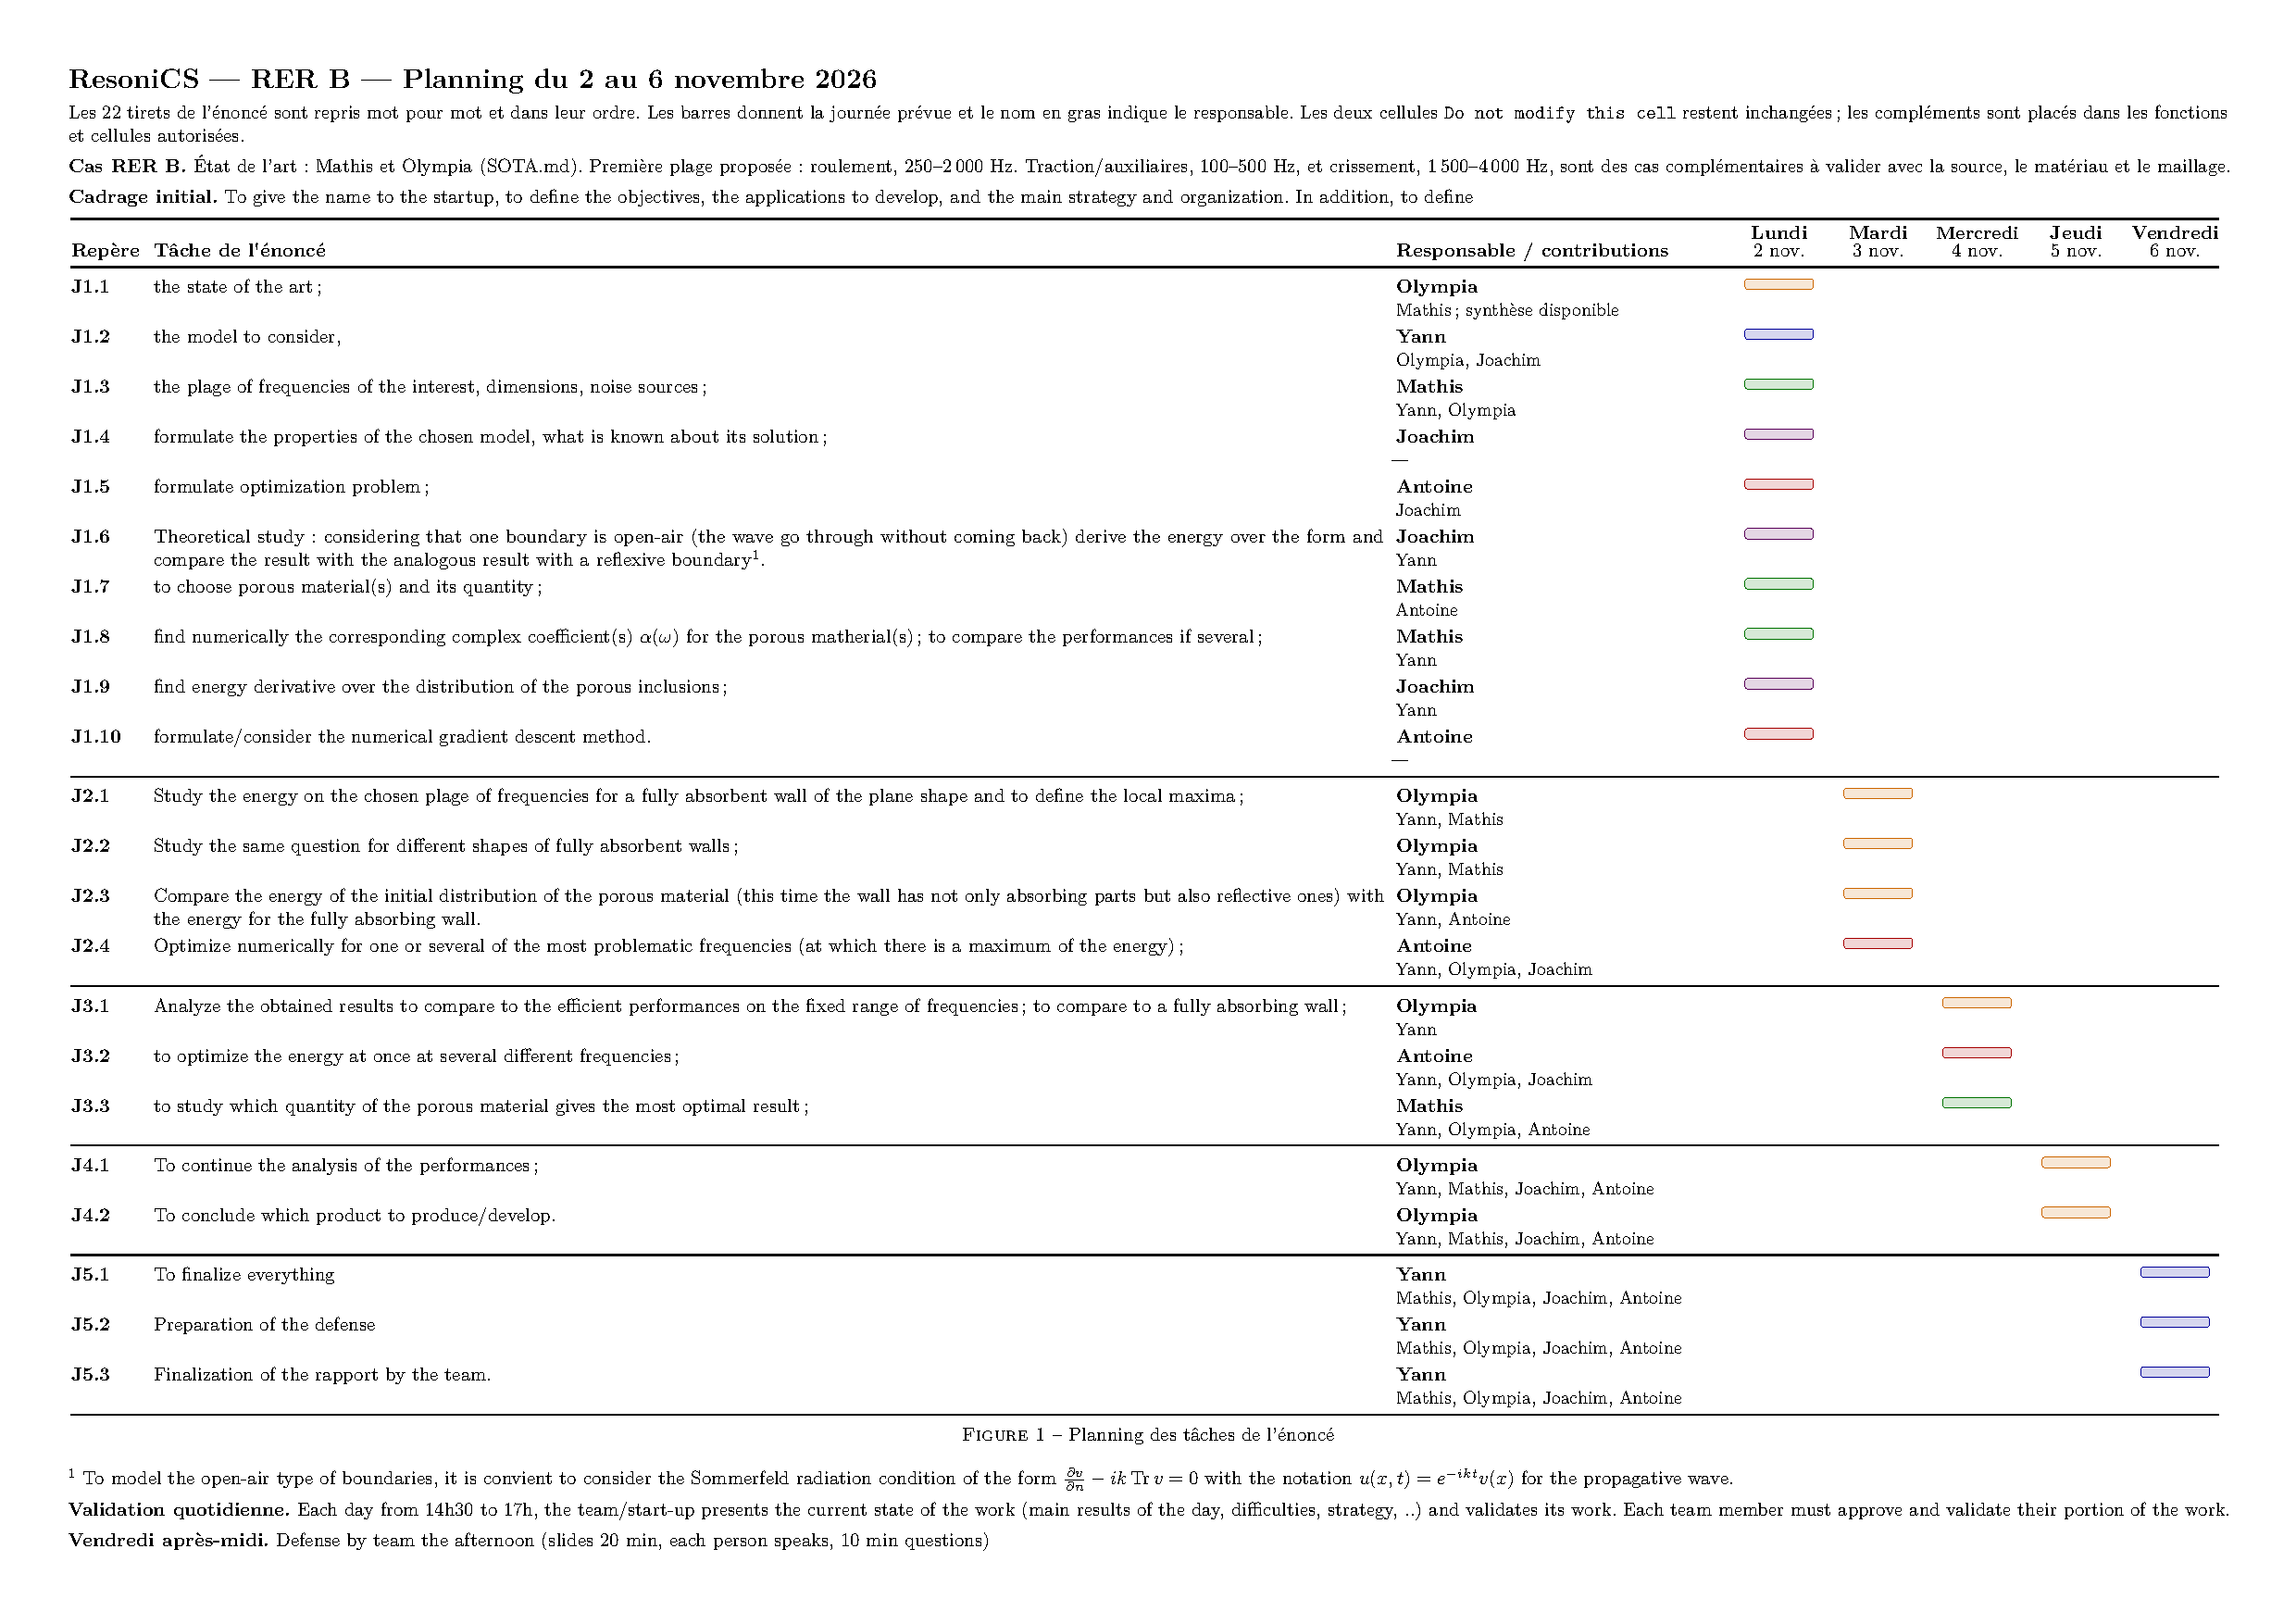
\includepdf[pages=1,fitpaper=true,addtotoc={1,section,1,Diagramme de Gantt,sec:gantt}]{gantt.pdf}
\section{Objectif et déroulement de la semaine}

ResoniCS réunit Yann, Mathis et Olympia, de la voie numérique, avec Joachim et Antoine, de la voie théorique. Le projet porte sur la recherche numérique d'une forme de mur et d'une répartition d'inclusions poreuses pour réduire le critère de pression du sujet, dans les conditions défavorables d'un tunnel réfléchissant. Les applications visées sont le bruit routier et le bruit ferroviaire.

Le planning suit les journées de l'énoncé du lundi 2 au vendredi 6 novembre 2026. Ces dates constituent le calendrier prévisionnel de cette semaine. Les résultats de chaque lot doivent être présentables avant le créneau quotidien de validation, compris entre 14h30 et 17h. Le vendredi après-midi est consacré à la soutenance de vingt minutes, suivie de dix minutes de questions. Chaque personne intervient et valide la partie dont elle est responsable.

\subsection{Répartition des cinq fichiers}

\begin{table}[H]\centering\small
\begin{tabularx}{\textwidth}{@{}>{\raggedright\arraybackslash}X>{\raggedright\arraybackslash}X>{\raggedright\arraybackslash}X>{\raggedright\arraybackslash}X@{}}
\toprule
Responsable & Voie & Fichier principal & Objet \\
\midrule
Yann & Numérique & {\small\ttfamily resonics.py} & Solveur, adaptation et intégration \\
Mathis & Numérique & {\small\ttfamily materiaux.py} & Matériaux, unités et bandes \\
Olympia & Numérique & {\small\ttfamily campagnes.py} & Expériences, comparaisons et figures \\
Joachim & Théorique & {\small\ttfamily objectif.py} & Objectif, adjoint et gradient \\
Antoine & Théorique & {\small\ttfamily optimisation.py} & Projection et descente \\
\bottomrule
\end{tabularx}\end{table}

Les fiches individuelles sont autonomes. Chacun peut écrire et vérifier son fichier avec les seules interfaces décrites dans sa fiche. Les fonctions qui ne sont pas encore disponibles sont remplacées, pour les vérifications seulement, par de petits cas synthétiques présents dans ce même fichier. Yann effectue ensuite l'intégration. Les noms pédagogiques {\small\ttfamily \nolinkurl{your_compute_objective_function}} et {\small\ttfamily \nolinkurl{your_optimization_procedure}} restent attribués aux deux membres de la voie théorique.

\subsection{Jalons et dépendances}

\begin{itemize}
\item \textbf{Lundi, Y1/M1/O1/J1/A1.} Fixer les conventions, la source, les dimensions, les bandes et le budget ; obtenir une loi de matériau documentée ; geler les signatures ; vérifier les petits cas, la projection et l'adjoint.
\item \textbf{Mardi, Y2/M2/O2/J2/A2.} Calculer les références entièrement recouvertes, repérer les pics, vérifier le gradient par différences centrées, puis mener une première optimisation monofréquence.
\item \textbf{Mercredi, Y3/M3/O3/J3/A3.} Optimiser une distribution commune à plusieurs fréquences, comparer plusieurs budgets, puis contrôler la bande et le raffinement.
\item \textbf{Jeudi, Y4/M4/O4/J4/A4.} Vérifier la reproductibilité, la stabilité du classement et les contraintes de réalisation ; choisir le produit dans la famille étudiée ; figer les données et les figures.
\item \textbf{Vendredi, Y5/M5/O5/J5/A5.} Finaliser les documents, vérifier le rendu et répéter à cinq avant la soutenance.
\end{itemize}

Les développements de lundi sont parallèles grâce aux contrats. L'optimisation acoustique dépend ensuite du solveur validé, de la loi complexe du matériau et du gradient contrôlé. La recommandation du jeudi dépend de la comparaison sur toute la bande et à quantité de poreux annoncée.

\subsection{Décisions à valider au premier point}

Le sujet laisse au groupe le choix des bandes route et rail, des dimensions, de la source précise et des matériaux. La table de coefficients d'absorption réels du document Filoche ne suffit pas à reconstruire une impédance complexe. Les anciens programmes ne fournissent pas non plus de fonction {\small\ttfamily \nolinkurl{compute_alpha}}. Mathis doit donc obtenir le modèle et ses paramètres, ou une table d'impédances avec sa provenance, afin de produire un coefficient physique utilisable.

Le programme de support emploie un coefficient Robin dont le signe doit être relié explicitement à celui de la condition physique. Yann et Joachim valident cette correspondance sur un cas plan. Les formules de gradient du cahier sont dérivées du système réellement assemblé, puis contrôlées par perturbations du coût.

L'EI impose une quantité de matériau, ce qui conduit ici à un budget de longueur absorbante pondérée, à épaisseur et profondeur fixées. L'aire unité conservée dans la partie trois précédente ne devient pas une contrainte de ce projet. Les comparaisons emploient une même source, des dimensions de référence annoncées et un budget absolu commun entre les formes.

Pour la comparaison théorique ouverte/réfléchissante, le premier scénario proposé conserve le bord source et ouvre une paroi latérale. Joachim fait valider le périmètre de l'étude demandée. Si une dérivée géométrique de forme est attendue, sa dérivation constitue un complément spécifique à la dérivée de densité détaillée ici.

\subsection{Ce qui est repris du travail antérieur}

Nous reprenons la démarche de vérification sur un cas connu, le suivi des résidus, le raffinement à géométrie fixée et les exports de résultats. Le modèle de l'EI utilise les différences finies et une condition Robin absorbante, avec une excitation de Dirichlet non homogène en haut. Les choix de source, de nombres d'onde et de conservation d'aire du devoir précédent restent liés à leurs propres énoncés.

Le générateur fourni permet de commencer avec les niveaux zéro, un et deux. Malgré le nom {\small\ttfamily \nolinkurl{create_motif_koch}}, il construit un motif orthogonal à huit segments de quart. Les descriptions et les figures doivent représenter ce contour effectif. La règle orale de détails d'ordre demi-longueur d'onde guide la conception ; l'énoncé exige au moins dix points par longueur d'onde. Ces deux contrôles ont des rôles différents.

\subsection{Documents et soutenance}

Le rapport est rédigé en LaTeX dans le template récent, article A4 de onze points avec marges de deux virgule deux centimètres. La présentation reprend Beamer CambridgeUS en seize neuvièmes, un plan détaillé et des rappels de plan. Les paragraphes expliquent les choix, les figures portent des légendes nominales et les grandeurs numériques proviennent des exports.

Une première répartition orale réserve quatre minutes à chacun : modèle et calcul pour Yann, matériau et bandes pour Mathis, critère et gradient pour Joachim, optimisation pour Antoine, comparaisons et produit pour Olympia. La répétition permet d'ajuster les transitions en conservant vingt minutes au total.

Chaque membre remet son fichier, les contrôles exécutés, ses paramètres et les éléments d'analyse de son lot. Il relit et approuve les figures et les équations correspondantes avant la validation collective.
\section{Contrat commun ResoniCS}

Cinq fichiers à produire, un seul fichier à écrire par personne : Yann {\small\ttfamily resonics.py}, Mathis {\small\ttfamily materiaux.py}, Olympia {\small\ttfamily campagnes.py}, Joachim {\small\ttfamily objectif.py}, Antoine {\small\ttfamily optimisation.py}. Chaque fichier possède un petit exemple autonome sous {\small\ttfamily if \nolinkurl{__name__} == \nolinkurl{"__main__":}}. Les essais de fonctions emploient de petits exemples explicitement synthétiques ; ils ne sont jamais publiés comme performances acoustiques. NumPy, SciPy, Matplotlib et bibliothèque standard uniquement. Commentaires en phrases françaises sans équations ni symboles mathématiques. Les équations restent dans les explications et les calculs Python. Les signatures ci-dessous sont des contrats proposés, pas des fonctions déjà présentes dans le support.

Le support distribué reste conservé. Yann écrit l'adaptation et les appels, sans demander aux autres d'éditer les modules fournis. Les noms pédagogiques {\small\ttfamily \nolinkurl{your_compute_objective_function}} et {\small\ttfamily \nolinkurl{your_optimization_procedure}} sont conservés. Si l'appel long du programme distribué est gardé, son adaptation aux nouveaux arguments est faite dans {\small\ttfamily resonics.py}, hors des blocs signalés comme imposés.

\subsection{Unités et signes}

La fréquence publique {\small\ttfamily \nolinkurl{frequency_hz}} est en hertz. On définit la pulsation {\small\ttfamily \nolinkurl{angular_frequency_rad_s} = \nolinkurl{2*pi*frequency_hz}}, puis {\small\ttfamily \nolinkurl{k_per_m} = \nolinkurl{angular_frequency_rad_s} / \nolinkurl{c_m_s}} et la longueur d'onde {\small\ttfamily \nolinkurl{wavelength_m} = \nolinkurl{c_m_s} / \nolinkurl{frequency_hz}}. Le paramètre historique {\small\ttfamily omega} de {\small\ttfamily \nolinkurl{processing.solve_helmholtz}} reçoit en réalité \textbf{le nombre d'onde}, jamais directement les hertz ou la pulsation.

Convention temporelle : exp(-i*omega*t). Avec normale sortante, la Robin physique s'écrit {\small\ttfamily \nolinkurl{partial_n} u + \nolinkurl{a_phys*u} = 0}. Le support élimine la valeur de bord par {\small\ttfamily \nolinkurl{u_B} = \nolinkurl{u_I/(1-h*a_code)}} lorsque les coefficients imposés valent un et le second membre Robin est nul. Il représente donc {\small\ttfamily \nolinkurl{partial_n} u - \nolinkurl{a_code*u} = 0}. On utilise {\small\ttfamily \nolinkurl{a_code} = \nolinkurl{-a_phys}}. Pour une impédance de surface documentée {\small\ttfamily \nolinkurl{Z_s} = \nolinkurl{pression/vitesse_normale_sortante}}, {\small\ttfamily \nolinkurl{a_code} = \nolinkurl{i*omega*rho_air/Z_s}}. Sommerfeld correspond à {\small\ttfamily \nolinkurl{a_code} = i*k}. Une vérification sur onde plane et un contrôle de passivité précèdent toute conclusion physique. La constante {\small\ttfamily 10-10j} du démo n'identifie aucun matériau réel.

\subsection{Conception et quantité}

La densité {\small\ttfamily chi} est un vecteur réel de taille B, borné entre zéro et un, associé uniquement aux nœuds Robin du mur qui touchent au moins une face intérieure. Les Robin d'ouverture sont exclues de la conception. La géométrie reste fixée pendant une optimisation ; on compare les niveaux géométriques dans des optimisations séparées.

Pour chaque nœud de conception, {\small\ttfamily \nolinkurl{design_weights}} vaut le pas multiplié par le nombre de faces adjacentes au fluide, avec les mêmes faces que l'assemblage. Ce sont des longueurs discrètes en mètres, à confronter à la longueur du profil lors du raffinement. On impose {\small\ttfamily \nolinkurl{dot(design_weights,} chi) = \nolinkurl{material_length_m}}, budget absolu commun entre formes. Avec épaisseur et profondeur constantes, le volume poreux est proportionnel à cette longueur. La fraction nodale {\small\ttfamily \nolinkurl{V_obj}} du démo ne remplace pas ce budget. Le cas entièrement recouvert est une référence qui utilise généralement plus de matériau, pas une borne assurée du coût.

\subsection{Assemblage pour Joachim}

Yann fournit une fonction passée en argument :

\begin{Verbatim}[breaklines,breakanywhere,fontsize=\footnotesize]
assemble(chi, frequency_hz) -> {
    "A": matrice creuse complexe de taille (n, n),
    "b": vecteur complexe de taille (n,),
    "cell_weights": vecteur réel positif de taille (n,),
    "face_rows": indices entiers de taille (n_faces,),
    "face_design": indices de conception de taille (n_faces,),
    "dA_diag": valeurs complexes de taille (n_faces,)
}
\end{Verbatim}

{\small\ttfamily A} et {\small\ttfamily b} sont restreints aux nœuds intérieurs après élimination des bords avec le support. {\small\ttfamily \nolinkurl{cell_weights}} vaut le carré du pas. Chaque entrée de face apporte une dérivée diagonale de {\small\ttfamily A} à la ligne {\small\ttfamily \nolinkurl{face_rows}}, relativement à la variable {\small\ttfamily \nolinkurl{chi[face_design]}}. Les répétitions sont conservées si un nœud Robin touche plusieurs intérieurs. Dans le cas imposé de coefficients unitaires et de second membre Robin nul, la valeur de face est {\small\ttfamily \nolinkurl{h*Alpha_code/(1-h*Alpha_code*chi_l)**2}}. {\small\ttfamily b} ne dépend pas de la densité. Tout changement de cette dernière hypothèse demande de compléter la dérivée du second membre.

Joachim fournit :

\begin{Verbatim}[breaklines,breakanywhere,fontsize=\footnotesize]
your_compute_objective_function(domain_omega, u, spacestep) -> float
evaluate_frequency(chi, frequency_hz, assemble, with_gradient=True) -> dict
evaluate_band(chi, frequencies_hz, frequency_weights, assemble,
              reference_energies=None, with_gradient=True) -> dict
\end{Verbatim}

L'objectif sur grille vaut le carré du pas multiplié par la somme des modules au carré \textbf{aux nœuds intérieurs}, dont le code fourni vaut moins un. Pour une fréquence : résoudre {\small\ttfamily A*U=b}, puis {\small\ttfamily \nolinkurl{A.conj().T*P=2*cell_weights*U}}. Le gradient réel euclidien s'obtient en ajoutant pour chaque face {\small\ttfamily \nolinkurl{-real(conj(P[row])*dA_diag*U[row])}} à la variable indiquée. La dépendance par Dirichlet non homogène est déjà dans le champ total et dans le second membre. On ne remplace pas le champ total par un champ homogénéisé dans le gradient.

{\small\ttfamily \nolinkurl{evaluate_band}} retourne au minimum {\small\ttfamily \{"value": float, "gradient": vecteur réel de taille B ou None, "energies": vecteur par fréquence, \nolinkurl{"state_residuals":} vecteur\}}. Les poids fréquentiels sont fixés, positifs ou nuls, et de somme un. Des énergies de référence strictement positives peuvent normaliser chaque fréquence, à condition d'être gelées avant optimisation et communes aux produits comparés. L'énergie définie ici est le critère de pression du sujet, pas directement une puissance dissipée.

\subsection{Appel d'optimisation pour Antoine}

Yann ferme les paramètres de bande dans un callback :

\begin{Verbatim}[breaklines,breakanywhere,fontsize=\footnotesize]
evaluate(chi, with_gradient=True) -> {
    "value": float,
    "gradient": vecteur réel de taille B ou None
}
\end{Verbatim}

Antoine fournit :

\begin{Verbatim}[breaklines,breakanywhere,fontsize=\footnotesize]
project_density(z, design_weights, material_length_m,
                tol=1e-10, max_iter=100) -> chi
your_optimization_procedure(chi0, evaluate, design_weights, material_length_m,
                            step0=1.0, max_iter=100,
                            feasibility_tol=1e-10, gradient_tol=1e-6,
                            armijo=1e-4, reduction=0.5, increase=1.1,
                            min_step=1e-12, max_backtracks=40) -> dict
\end{Verbatim}

Avec le gradient euclidien, la projection utilise {\small\ttfamily \nolinkurl{clip(z-lambda*design_weights,} 0, 1)} ; le décalage scalaire est trouvé par dichotomie pour respecter le budget pondéré. La descente utilise un retour arrière et le coût réellement recalculé après projection. La même densité sert à toutes les fréquences. Le retour contient densité finale, coût final, gradient final, historique sans lignes fictives, erreur de budget, résidu projeté et raison de l'arrêt. Une convergence locale ou une limite d'itérations n'est pas un certificat d'optimalité globale.

\subsection{Matériaux et campagnes}

Mathis fournit {\small\ttfamily \nolinkurl{compute_material_response(frequencies_hz,} \nolinkurl{material_parameters,} \nolinkurl{air_parameters)} -> dict} avec impédance complexe, coefficients Robin physique et code, domaine de validité, unités et provenance. Les courbes de coefficients d'absorption réels ne suffisent pas à identifier la phase d'une impédance complexe. Le modèle doit être documenté ou fourni par les enseignants ; l'absence de ce modèle est un point à lever lundi, pas une donnée à inventer.

Olympia reçoit les fonctions de construction, d'évaluation et d'optimisation comme arguments, donc son fichier n'importe pas les fichiers en cours de rédaction. Un cas transmis par Yann contient identifiant, métadonnées de géométrie/source, {\small\ttfamily \nolinkurl{design_weights}}, budget, densité initiale. {\small\ttfamily \nolinkurl{evaluate_case(case,} chi, \nolinkurl{frequency_hz)}} retourne énergie, champ complexe intérieur, coordonnées et masques, résidu, traces Robin par face et puissance dissipée si le coefficient physique est validé. {\small\ttfamily \nolinkurl{optimize_case(case,} \nolinkurl{frequencies_hz,} \nolinkurl{frequency_weights,} chi0)} retourne le dictionnaire d'Antoine.

Les bandes route et rail, dimensions, lois de matériau et budget sont des choix à documenter au premier jalon. À défaut d'une pondération spectrale documentée, une pondération uniforme est annoncée comme telle. La règle d'au moins dix points par longueur d'onde vient du sujet ; l'échelle d'irrégularité proche de la demi-longueur d'onde est une règle de conception donnée oralement, à tester. Aucune performance de produit n'est déjà acquise.

\subsection{Clés de retour retenues pour la première intégration}

Le dictionnaire de {\small\ttfamily \nolinkurl{your_optimization_procedure}} emploie les mêmes clés dans les cinq lots :

\begin{Verbatim}[breaklines,breakanywhere,fontsize=\footnotesize]
{
    "chi": densite_finale,
    "value": cout_final,
    "gradient": gradient_final,
    "history": historique,
    "budget_error": erreur_absolue_de_budget,
    "projected_gradient_norm": residu_projete,
    "stop_reason": motif_arret,
    "converged": convergence_annoncee,
    "n_iterations": iterations_acceptees,
    "n_evaluations": appels_evaluation,
}
\end{Verbatim}

{\small\ttfamily history} est une liste de dictionnaires avec {\small\ttfamily iteration}, {\small\ttfamily value}, {\small\ttfamily step}, {\small\ttfamily \nolinkurl{projected_gradient_norm}}, {\small\ttfamily \nolinkurl{budget_error}} et {\small\ttfamily backtracks}. La ligne initiale a le numéro zéro et un pas nul. Les clés supplémentaires sont autorisées, mais ces noms restent communs.

\subsection{Clés des callbacks de campagne}

Les clés suivantes sont retenues pour la première intégration. Un cas construit par {\small\ttfamily \nolinkurl{build_case(specification)}} contient {\small\ttfamily \nolinkurl{case_id}}, {\small\ttfamily \nolinkurl{design_weights}}, {\small\ttfamily \nolinkurl{material_length_m}}, {\small\ttfamily chi0} et {\small\ttfamily metadata}. Les métadonnées contiennent au minimum {\small\ttfamily level}, {\small\ttfamily \nolinkurl{spacestep_m}}, {\small\ttfamily \nolinkurl{c_m_s}}, {\small\ttfamily geometry}, {\small\ttfamily source} et {\small\ttfamily material}.

{\small\ttfamily \nolinkurl{evaluate_case(case,} chi, \nolinkurl{frequency_hz)}} renvoie {\small\ttfamily energy}, {\small\ttfamily u}, {\small\ttfamily coordinates}, {\small\ttfamily masks}, {\small\ttfamily \nolinkurl{relative_residual}}, {\small\ttfamily \nolinkurl{robin_traces}} et {\small\ttfamily \nolinkurl{dissipated_power}}. Le champ {\small\ttfamily u} est un tableau complexe de la même forme que la grille. {\small\ttfamily coordinates} contient {\small\ttfamily x}, les abscisses des colonnes, et {\small\ttfamily y}, les ordonnées des lignes. {\small\ttfamily masks} contient {\small\ttfamily interior}, {\small\ttfamily design} et {\small\ttfamily open}, tableaux booléens de la forme de la grille. {\small\ttfamily \nolinkurl{robin_traces}} conserve une valeur par face du mur et {\small\ttfamily \nolinkurl{dissipated_power}} vaut {\small\ttfamily None} tant qu'un bilan physique n'est pas disponible. L'énergie est calculée avec le seul masque intérieur. Les poids et l'ordre des faces sont fournis par le constructeur.

Le callback d'optimisation retourne les clés communes de l'optimiseur, sans les renommer.

Les paramètres d'air sont nommés {\small\ttfamily \nolinkurl{c_m_s}} et {\small\ttfamily \nolinkurl{rho_air_kg_m3}}. Le dictionnaire de matériau utilise {\small\ttfamily name}, {\small\ttfamily \nolinkurl{thickness_m}}, {\small\ttfamily model}, {\small\ttfamily parameters}, {\small\ttfamily \nolinkurl{valid_frequency_hz}} et {\small\ttfamily provenance}. Le modèle ou les tables complexes sont décrits dans {\small\ttfamily parameters}. La première intégration retient les clés de sortie indiquées dans la fiche de Mathis.
\section{Yann — Voie numérique, solveur et intégration de ResoniCS}

Les repères \textbf{Y1 à Y5} du Gantt correspondent aux cinq journées, du lundi au vendredi.

\subsection{Livrable unique et responsabilité}

\textbf{Un seul fichier Python à produire : `resonics.py`.} Il constitue le point d'entrée du projet, adapte le support distribué et relie les quatre contributions {\small\ttfamily materiaux.py}, {\small\ttfamily objectif.py}, {\small\ttfamily optimisation.py} et {\small\ttfamily campagnes.py}. Les programmes du dossier de support sont conservés pour permettre les comparaisons. Les corrections ou adaptations nécessaires sont écrites dans {\small\ttfamily resonics.py}, sans demander aux autres membres de modifier les fichiers fournis.

Le fichier doit pouvoir exécuter ses petits contrôles avec le support seul, même lorsque les autres contributions ne sont pas encore disponibles. On effectue donc les imports des contributions au moment des commandes qui en ont besoin. Les exemples de contrôle sont explicitement synthétiques et restent distincts des données des applications route et rail.

Yann coordonne également la cohérence des unités, des paramètres et des résultats exportés, puis la compilation du rapport et de la présentation. Les membres valident eux-mêmes les éléments qu'ils présentent. Les résultats antérieurs de maillage et de FEM servent de méthode de travail et de vérification, et ne sont pas repris comme performances du produit ResoniCS.


\subsection{Contrat commun intégral à respecter}

Cinq fichiers à produire, un seul fichier à écrire par personne : Yann {\small\ttfamily resonics.py}, Mathis {\small\ttfamily materiaux.py}, Olympia {\small\ttfamily campagnes.py}, Joachim {\small\ttfamily objectif.py}, Antoine {\small\ttfamily optimisation.py}. Chaque fichier possède un petit exemple autonome sous {\small\ttfamily if \nolinkurl{__name__} == \nolinkurl{"__main__":}}. Les essais de fonctions emploient de petits exemples explicitement synthétiques ; ils ne sont jamais publiés comme performances acoustiques. NumPy, SciPy, Matplotlib et bibliothèque standard uniquement. Commentaires en phrases françaises sans équations ni symboles mathématiques. Les équations restent dans les explications et les calculs Python. Les signatures ci-dessous sont des contrats proposés, pas des fonctions déjà présentes dans le support.

Le support distribué reste conservé. Yann écrit l'adaptation et les appels, sans demander aux autres d'éditer les modules fournis. Les noms pédagogiques {\small\ttfamily \nolinkurl{your_compute_objective_function}} et {\small\ttfamily \nolinkurl{your_optimization_procedure}} sont conservés. Si l'appel long du programme distribué est gardé, son adaptation aux nouveaux arguments est faite dans {\small\ttfamily resonics.py}, hors des blocs signalés comme imposés.

\subsubsection{Unités et signes}

La fréquence publique {\small\ttfamily \nolinkurl{frequency_hz}} est en hertz. On définit la pulsation {\small\ttfamily \nolinkurl{angular_frequency_rad_s} = \nolinkurl{2*pi*frequency_hz}}, puis {\small\ttfamily \nolinkurl{k_per_m} = \nolinkurl{angular_frequency_rad_s} / \nolinkurl{c_m_s}} et la longueur d'onde {\small\ttfamily \nolinkurl{wavelength_m} = \nolinkurl{c_m_s} / \nolinkurl{frequency_hz}}. Le paramètre historique {\small\ttfamily omega} de {\small\ttfamily \nolinkurl{processing.solve_helmholtz}} reçoit en réalité \textbf{le nombre d'onde}, jamais directement les hertz ou la pulsation.

Convention temporelle : exp(-i*omega*t). Avec normale sortante, la Robin physique s'écrit {\small\ttfamily \nolinkurl{partial_n} u + \nolinkurl{a_phys*u} = 0}. Le support élimine la valeur de bord par {\small\ttfamily \nolinkurl{u_B} = \nolinkurl{u_I/(1-h*a_code)}} lorsque les coefficients imposés valent un et le second membre Robin est nul. Il représente donc {\small\ttfamily \nolinkurl{partial_n} u - \nolinkurl{a_code*u} = 0}. On utilise {\small\ttfamily \nolinkurl{a_code} = \nolinkurl{-a_phys}}. Pour une impédance de surface documentée {\small\ttfamily \nolinkurl{Z_s} = \nolinkurl{pression/vitesse_normale_sortante}}, {\small\ttfamily \nolinkurl{a_code} = \nolinkurl{i*omega*rho_air/Z_s}}. Sommerfeld correspond à {\small\ttfamily \nolinkurl{a_code} = i*k}. Une vérification sur onde plane et un contrôle de passivité précèdent toute conclusion physique. La constante {\small\ttfamily 10-10j} du démo n'identifie aucun matériau réel.

\subsubsection{Conception et quantité}

La densité {\small\ttfamily chi} est un vecteur réel de taille B, borné entre zéro et un, associé uniquement aux nœuds Robin du mur qui touchent au moins une face intérieure. Les Robin d'ouverture sont exclues de la conception. La géométrie reste fixée pendant une optimisation ; on compare les niveaux géométriques dans des optimisations séparées.

Pour chaque nœud de conception, {\small\ttfamily \nolinkurl{design_weights}} vaut le pas multiplié par le nombre de faces adjacentes au fluide, avec les mêmes faces que l'assemblage. Ce sont des longueurs discrètes en mètres, à confronter à la longueur du profil lors du raffinement. On impose {\small\ttfamily \nolinkurl{dot(design_weights,} chi) = \nolinkurl{material_length_m}}, budget absolu commun entre formes. Avec épaisseur et profondeur constantes, le volume poreux est proportionnel à cette longueur. La fraction nodale {\small\ttfamily \nolinkurl{V_obj}} du démo ne remplace pas ce budget. Le cas entièrement recouvert est une référence qui utilise généralement plus de matériau, pas une borne assurée du coût.

\subsubsection{Assemblage pour Joachim}

Yann fournit une fonction passée en argument :

\begin{Verbatim}[breaklines,breakanywhere,fontsize=\footnotesize]
assemble(chi, frequency_hz) -> {
    "A": matrice creuse complexe de taille (n, n),
    "b": vecteur complexe de taille (n,),
    "cell_weights": vecteur réel positif de taille (n,),
    "face_rows": indices entiers de taille (n_faces,),
    "face_design": indices de conception de taille (n_faces,),
    "dA_diag": valeurs complexes de taille (n_faces,)
}
\end{Verbatim}

{\small\ttfamily A} et {\small\ttfamily b} sont restreints aux nœuds intérieurs après élimination des bords avec le support. {\small\ttfamily \nolinkurl{cell_weights}} vaut le carré du pas. Chaque entrée de face apporte une dérivée diagonale de {\small\ttfamily A} à la ligne {\small\ttfamily \nolinkurl{face_rows}}, relativement à la variable {\small\ttfamily \nolinkurl{chi[face_design]}}. Les répétitions sont conservées si un nœud Robin touche plusieurs intérieurs. Dans le cas imposé de coefficients unitaires et de second membre Robin nul, la valeur de face est {\small\ttfamily \nolinkurl{h*Alpha_code/(1-h*Alpha_code*chi_l)**2}}. {\small\ttfamily b} ne dépend pas de la densité. Tout changement de cette dernière hypothèse demande de compléter la dérivée du second membre.

Joachim fournit :

\begin{Verbatim}[breaklines,breakanywhere,fontsize=\footnotesize]
your_compute_objective_function(domain_omega, u, spacestep) -> float
evaluate_frequency(chi, frequency_hz, assemble, with_gradient=True) -> dict
evaluate_band(chi, frequencies_hz, frequency_weights, assemble,
              reference_energies=None, with_gradient=True) -> dict
\end{Verbatim}

L'objectif sur grille vaut le carré du pas multiplié par la somme des modules au carré \textbf{aux nœuds intérieurs}, dont le code fourni vaut moins un. Pour une fréquence : résoudre {\small\ttfamily A*U=b}, puis {\small\ttfamily \nolinkurl{A.conj().T*P=2*cell_weights*U}}. Le gradient réel euclidien s'obtient en ajoutant pour chaque face {\small\ttfamily \nolinkurl{-real(conj(P[row])*dA_diag*U[row])}} à la variable indiquée. La dépendance par Dirichlet non homogène est déjà dans le champ total et dans le second membre. On ne remplace pas le champ total par un champ homogénéisé dans le gradient.

{\small\ttfamily \nolinkurl{evaluate_band}} retourne au minimum {\small\ttfamily \{"value": float, "gradient": vecteur réel de taille B ou None, "energies": vecteur par fréquence, \nolinkurl{"state_residuals":} vecteur\}}. Les poids fréquentiels sont fixés, positifs ou nuls, et de somme un. Des énergies de référence strictement positives peuvent normaliser chaque fréquence, à condition d'être gelées avant optimisation et communes aux produits comparés. L'énergie définie ici est le critère de pression du sujet, pas directement une puissance dissipée.

\subsubsection{Appel d'optimisation pour Antoine}

Yann ferme les paramètres de bande dans un callback :

\begin{Verbatim}[breaklines,breakanywhere,fontsize=\footnotesize]
evaluate(chi, with_gradient=True) -> {
    "value": float,
    "gradient": vecteur réel de taille B ou None
}
\end{Verbatim}

Antoine fournit :

\begin{Verbatim}[breaklines,breakanywhere,fontsize=\footnotesize]
project_density(z, design_weights, material_length_m,
                tol=1e-10, max_iter=100) -> chi
your_optimization_procedure(chi0, evaluate, design_weights, material_length_m,
                            step0=1.0, max_iter=100,
                            feasibility_tol=1e-10, gradient_tol=1e-6,
                            armijo=1e-4, reduction=0.5, increase=1.1,
                            min_step=1e-12, max_backtracks=40) -> dict
\end{Verbatim}

Avec le gradient euclidien, la projection utilise {\small\ttfamily \nolinkurl{clip(z-lambda*design_weights,} 0, 1)} ; le décalage scalaire est trouvé par dichotomie pour respecter le budget pondéré. La descente utilise un retour arrière et le coût réellement recalculé après projection. La même densité sert à toutes les fréquences. Le retour contient densité finale, coût final, gradient final, historique sans lignes fictives, erreur de budget, résidu projeté et raison de l'arrêt. Une convergence locale ou une limite d'itérations n'est pas un certificat d'optimalité globale.

\subsubsection{Matériaux et campagnes}

Mathis fournit {\small\ttfamily \nolinkurl{compute_material_response(frequencies_hz,} \nolinkurl{material_parameters,} \nolinkurl{air_parameters)} -> dict} avec impédance complexe, coefficients Robin physique et code, domaine de validité, unités et provenance. Les courbes de coefficients d'absorption réels ne suffisent pas à identifier la phase d'une impédance complexe. Le modèle doit être documenté ou fourni par les enseignants ; l'absence de ce modèle est un point à lever lundi, pas une donnée à inventer.

Olympia reçoit les fonctions de construction, d'évaluation et d'optimisation comme arguments, donc son fichier n'importe pas les fichiers en cours de rédaction. Un cas transmis par Yann contient identifiant, métadonnées de géométrie/source, {\small\ttfamily \nolinkurl{design_weights}}, budget, densité initiale. {\small\ttfamily \nolinkurl{evaluate_case(case,} chi, \nolinkurl{frequency_hz)}} retourne énergie, champ complexe intérieur, coordonnées et masques, résidu, traces Robin par face et puissance dissipée si le coefficient physique est validé. {\small\ttfamily \nolinkurl{optimize_case(case,} \nolinkurl{frequencies_hz,} \nolinkurl{frequency_weights,} chi0)} retourne le dictionnaire d'Antoine.

Les bandes route et rail, dimensions, lois de matériau et budget sont des choix à documenter au premier jalon. À défaut d'une pondération spectrale documentée, une pondération uniforme est annoncée comme telle. La règle d'au moins dix points par longueur d'onde vient du sujet ; l'échelle d'irrégularité proche de la demi-longueur d'onde est une règle de conception donnée oralement, à tester. Aucune performance de produit n'est déjà acquise.

\subsection{Signatures fournies et organisation du fichier}

Le contrat ci-dessus est complet. Les fonctions {\small\ttfamily assemble}, {\small\ttfamily \nolinkurl{evaluate_case}}, {\small\ttfamily \nolinkurl{optimize_case}} et le callback {\small\ttfamily evaluate} sont fournis aux autres contributions par le coordinateur. Les signatures des fonctions rédigées par Mathis, Joachim et Antoine sont reprises sans renommer leurs paramètres. Les fonctions d'Olympia reçoivent les callbacks, ce qui leur permet de fonctionner sans importer les contributions encore en rédaction.

L'architecture interne de {\small\ttfamily resonics.py} peut suivre cet ordre : imports standard et scientifiques, paramètres et étiquettes, chargement du support, construction d'un cas, numérotation des inconnues et des faces, assemblage réduit, reconstruction du champ et des traces, contrôles, raccordement aux contributions, exports, puis interface en ligne de commande. Les noms des aides internes sont libres ; leurs sorties doivent aboutir exactement aux contrats communs.

\textbf{Entrées physiques à fixer explicitement au premier jalon :} vitesse du son en mètres par seconde, masse volumique de l'air, dimensions en mètres, source imposée et son unité, liste de fréquences en hertz, modèle matériau avec sa provenance et ses hypothèses, niveau géométrique, pas en mètres et quantité absolue de matériau. Une valeur présente dans le démonstrateur ne constitue pas à elle seule une donnée matériau ou une donnée de bruit routier ou ferroviaire.

\textbf{Métadonnées à conserver pour chaque cas :} identifiant stable, scénario, dimensions, pas, niveau, nombre de nœuds intérieurs, nombre de variables de conception, liste des faces de conception, poids de conception, longueur du profil, longueur discrète des faces et budget. Les métadonnées décrivent aussi la position des bords et la convention d'orientation des coordonnées.

\subsection{Étapes de réalisation}

\subsubsection{Établir la référence du support avant toute adaptation}

\begin{enumerate}
\item Lire le démonstrateur et les fonctions appelées dans {\small\ttfamily preprocessing.py}, {\small\ttfamily processing.py}, {\small\ttfamily postprocessing.py} et {\small\ttfamily \nolinkurl{_env.py}}. Conserver les fichiers distribués et noter leurs empreintes pour savoir quelle version sert de référence.
\item Identifier les blocs signalés comme imposés dans le démonstrateur et conserver leur contenu. L'adaptation et les appels sont placés dans {\small\ttfamily resonics.py}, hors de ces blocs.
\item Relever les étiquettes : intérieur moins un, extérieur complémentaire moins deux, Dirichlet un, Neumann deux et Robin trois. Les masques sont toujours construits à partir de ces étiquettes, jamais à partir d'un test approximatif sur la couleur d'un graphique.
\item Vérifier la convention de numérotation complète du support : la case de ligne et colonne de grille est aplatie avec la largeur du tableau, et non sa hauteur. Conserver une correspondance dans les deux sens entre cet indice complet et l'indice intérieur réduit.
\item Exécuter un petit cas plan sans optimisation. Noter les paramètres effectivement employés et les grandeurs renvoyées. Le support n'affiche et ne renvoie le champ que sur les nœuds intérieurs ; ses zéros de bord ne sont donc pas des traces de pression calculées.
\item Relever les éléments à compléter dans le démonstrateur : objectif initial nul, boucle pédagogique contenant des variables non définies si elle est activée, appel d'objectif dont le nom diffère du nom pédagogique, et invocation de l'optimisation commentée. Les fonctions de Joachim et Antoine seront raccordées par le coordinateur. Ne pas présenter ces points comme déjà corrigés.
\item Vérifier les fonctions auxiliaires avant de les appeler. Certaines fonctions de traitement de bord ou de coloriage non employées par le chemin principal font référence à des noms non définis dans {\small\ttfamily \nolinkurl{_env.py}} ou dans leur module. On peut conserver ces fonctions inutilisées sans prétendre les avoir validées.
\end{enumerate}

\subsubsection{Construire et contrôler les géométries et leurs unités}

\begin{enumerate}
\item Appeler le générateur fourni en conservant sa définition du motif et en faisant d'abord varier le niveau. Le nom {\small\ttfamily \nolinkurl{create_motif_koch}} désigne ici un motif de huit segments au quart et des rotations à angle droit. Il faut montrer et décrire ce motif réel, plutôt que reprendre le Koch triangulaire à quatre segments au tiers du précédent projet.
\item Définir des coordonnées physiques à partir des indices et du pas. Préciser si l'ordonnée augmente vers le bas de la grille ou vers le haut du dessin. Les normales sortantes sont déterminées à partir du fluide et du bord considéré, indépendamment du sens d'affichage.
\item Vérifier que les nœuds intérieurs ne touchent jamais le bord extérieur du tableau. Les stencils accèdent aux quatre voisins ; une case intérieure sur ce bord pourrait utiliser un indice négatif ou sortir du tableau. Vérifier aussi la connexion de la région fluide, l'absence d'ouvertures involontaires et l'appartenance de chaque bord à une catégorie explicite.
\item Examiner la partition obtenue à chaque niveau. Les branches de la routine de partitionnement utilisent des indices de ligne et de colonne différents ; un domaine rectangulaire ne permet pas d'intervertir leurs bornes. Un nouveau test doit porter sur les dimensions réellement choisies. On signale un cas invalide au lieu de le corriger silencieusement.
\item Au niveau géométrique fixé, construire au moins deux résolutions qui représentent les mêmes sommets et les mêmes dimensions physiques. Les pas successifs subdivisent les segments existants. Le contrôle porte sur les coordonnées et le profil, pas seulement sur le numéro du niveau.
\item Vérifier la règle du sujet à la fréquence maximale. Avec {\small\ttfamily \nolinkurl{wavelength_min_m} = \nolinkurl{c_m_s} / \nolinkurl{max(frequencies_hz)}}, on impose au moins dix points par longueur d'onde, donc un pas au plus égal au dixième de cette longueur. Le nombre de points, le nombre d'intervalles et la longueur physique ne sont pas interchangeables ; les bornes réelles du tableau doivent être calculées.
\item Vérifier séparément la représentation des plus petits motifs. Le générateur emploie des subdivisions puis des conversions en entiers ; un segment plus court que la maille peut disparaître. Choisir des dimensions et subdivisions compatibles, vérifier que les sommets existent après discrétisation et refuser les niveaux non résolus. Au besoin, fixer plusieurs mailles par plus petit segment et tester une résolution supérieure.
\item Comparer la taille physique des irrégularités à la demi-longueur d'onde dans la bande visée. Cette règle donnée oralement est une piste de conception à tester. Elle ne remplace pas le critère de résolution de la longueur d'onde ni le contrôle des motifs les plus fins.
\end{enumerate}

\subsubsection{Construire les variables de conception et compter les faces}

\begin{enumerate}
\item Séparer le mur à optimiser des éventuelles frontières ouvertes. Ces deux ensembles peuvent porter une étiquette Robin, mais seuls les nœuds du mur appartiennent à la conception. Une frontière ouverte conserve son coefficient et ne reçoit aucune part du budget de matériau.
\item Parcourir les quatre voisins de chaque nœud intérieur. Pour chaque voisin appartenant au mur Robin, enregistrer une face avec l'indice intérieur réduit, l'indice du nœud de bord, la direction et l'indice de la variable de conception correspondante. L'ordre de ce relevé est déterministe.
\item Conserver une seule variable de densité par nœud de conception, mais une entrée par face. Un nœud Robin peut toucher plusieurs nœuds intérieurs et doit alors apparaître plusieurs fois dans la liste des faces. Ne pas supprimer ces répétitions par une opération sur les indices de conception.
\item Définir les poids de conception en additionnant le pas sur les faces associées à chaque variable. La somme des poids est la longueur de contact discrète entre le mur et le fluide. La comparer à la longueur du profil fourni et suivre leur évolution pendant le raffinement, notamment aux coins.
\item Vérifier le budget absolu et sa faisabilité. La quantité de matériau demandée doit être comprise entre zéro et la somme des poids. Le cas « mur entièrement absorbant » correspond à la densité unitaire et peut employer davantage de matériau que les produits optimisés. Il sert de référence distincte et n'est pas une borne garantie de l'objectif.
\item Construire une densité initiale faisable ou la projeter avec la fonction d'Antoine dès qu'elle est disponible. Pour comparer les formes, garder le même budget physique et le même scénario source, plutôt qu'une même moyenne des valeurs nodales.
\end{enumerate}

\subsubsection{Assembler le problème réduit, avec les mêmes coefficients que le support}

\begin{enumerate}
\item Préparer les coefficients et seconds membres avec les routines distribuées. Le contrat commun de cette semaine porte sur les coefficients imposés unitaires et sur un second membre Robin nul. Vérifier ces hypothèses dans l'adaptation et refuser une généralisation silencieuse à des coefficients variables.
\item Construire les matrices complètes du support avec {\small\ttfamily \nolinkurl{compute_stiffness_matrix}} et {\small\ttfamily \nolinkurl{compute_mass_matrix}}, puis appliquer les conditions Dirichlet, Neumann et Robin dans le même ordre que {\small\ttfamily \nolinkurl{solve_helmholtz}}. Le coefficient de masse est multiplié par le carré du nombre d'onde, puisque la variable historique {\small\ttfamily omega} de cette fonction contient ce nombre d'onde.
\item Employer le champ total avec la donnée Dirichlet non homogène. Les contributions de cette donnée sont reportées dans le second membre. Ne pas annuler l'excitation lorsqu'on prépare l'adjoint et ne pas substituer au champ total une inconnue de relèvement homogène dans le contrat de Joachim.
\item Après traitement des bords, extraire les lignes et colonnes intérieures ainsi que le second membre intérieur. Convertir la matrice au format creux adapté à la factorisation et ramener le second membre à un vecteur unidimensionnel. La matrice complète contient des équations d'identité aux autres nœuds ; celles-ci ne doivent pas devenir des variables d'optimisation.
\item Fournir {\small\ttfamily \nolinkurl{cell_weights}} constant, égal au carré du pas sur les inconnues intérieures. Ce choix correspond au critère discret commun et doit être le même dans l'objectif et dans l'adjoint.
\item Pour chaque face du mur, poser le coefficient local comme le coefficient matériau de code multiplié par sa densité. Avec les hypothèses du contrat, l'élimination fournit une contribution diagonale correspondant à la trace divisée par le terme de Robin. Construire la dérivée de cette même contribution, sans reprendre une formule continue qui ne différencierait pas exactement le code.
\item La dérivée diagonale retournée par face est exactement :
\end{enumerate}

\begin{Verbatim}[breaklines,breakanywhere,fontsize=\footnotesize]
   dA_diag = h * Alpha_code / (1.0 - h * Alpha_code * chi[face_design])**2
\end{Verbatim}

   {\small\ttfamily \nolinkurl{face_rows}} et {\small\ttfamily \nolinkurl{face_design}} ont la même longueur que ce tableau. Les faces d'une ouverture fixe ne figurent pas dans ces trois tableaux de dérivées. Les répétitions sont conservées et seront additionnées par Joachim.
\begin{enumerate}
\item Vérifier que le second membre reste indépendant de la densité dans le cas retenu. Si un second membre Robin non nul ou une autre paramétrisation est ensuite introduit, il faut modifier et valider le contrat de dérivation avant de poursuivre les optimisations.
\item Contrôler tous les dénominateurs de Robin avant la résolution. Signaler un dénominateur trop petit, une matrice singulière, des valeurs non finies ou un résidu excessif, avec l'identifiant du cas et la fréquence. Ne pas enregistrer une énergie nulle comme remplacement d'une résolution échouée.
\end{enumerate}

\subsubsection{Vérifier le signe physique de Robin et les frontières ouvertes}

\begin{enumerate}
\item Établir explicitement le lien entre la Robin physique et son écriture dans le support. Pour une face dont le second membre est nul et les coefficients unitaires, la trace éliminée satisfait :
\end{enumerate}

\begin{Verbatim}[breaklines,breakanywhere,fontsize=\footnotesize]
   u_boundary_face = u_interior[face_row] / (1.0 - h * a_code_face)
\end{Verbatim}

   La différence entre la trace de bord et la valeur intérieure, divisée par le pas, représente la dérivée vers la normale sortante. Elle vaut ici le coefficient de code multiplié par la trace. Le signe est donc celui indiqué dans le contrat commun.
\begin{enumerate}
\item La fonction de Mathis reçoit des fréquences en hertz et renvoie une réponse matériau documentée. Yann convertit les unités à une seule interface, vérifie le coefficient physique et le coefficient de code, puis injecte uniquement le coefficient de code dans les routines du support. La constante complexe du démonstrateur reste un paramètre de contrôle, pas une identité de matériau.
\item Préparer le cas réfléchissant avec un coefficient Robin de code nul sur le mur, ce qui doit retrouver le comportement Neumann homogène. À la limite d'une densité nulle, les deux implémentations doivent donner les mêmes champs intérieurs.
\item Préparer un cas d'ouverture locale avec le coefficient de code égal au nombre d'onde multiplié par l'unité imaginaire. Il s'agit de l'approximation de Sommerfeld du premier ordre, à contrôler sur une onde sortante normale. Une ouverture fixe est exclue du budget et du gradient.
\item Pour comparer une frontière réfléchissante et une frontière ouverte, conserver la source, sa normalisation et les autres paramètres. Si l'ouverture remplace la frontière qui portait la source Dirichlet, imposer une condition incidente non homogène cohérente. Remplacer simplement cette source par une Sommerfeld homogène supprimerait l'excitation. La frontière modifiée et le choix de source doivent être approuvés au premier jalon avec la partie théorique.
\item Contrôler l'absorption et la réflexion sur un problème plan avant les géométries irrégulières. Avec une source unitaire en haut, un axe vertical orienté du haut vers le bas et un bas ouvert, la référence continue à incidence normale est une exponentielle qui se propage vers le bas. Pour le bas réfléchissant, une combinaison de cosinus satisfait la dérivée normale nulle, en évitant ses fréquences singulières. Le support est une approximation discrète de ces références ; l'écart doit diminuer avec le pas.
\item Ne pas transférer directement le calcul spectral réel du précédent projet au nouvel opérateur complexe. Une factorisation directe creuse constitue la référence pour les réponses d'état et d'adjoint. Le choix d'un autre solveur doit conserver les résidus et les mêmes équations.
\end{enumerate}

Pour rendre le contrôle plan directement programmable, on prend un rectangle de hauteur physique {\small\ttfamily H}, une profondeur {\small\ttfamily y} croissante du haut vers le bas, une pression unitaire en haut et Neumann sur les côtés. À nombre d'onde non nul, avec un coefficient de code constant {\small\ttfamily \nolinkurl{a_code}} en bas, la référence est :

\begin{Verbatim}[breaklines,breakanywhere,fontsize=\footnotesize]
u_reference = (
    numpy.cos(k * (H - y))
    - (a_code / k) * numpy.sin(k * (H - y))
) / (
    numpy.cos(k * H)
    - (a_code / k) * numpy.sin(k * H)
)
\end{Verbatim}

La hauteur {\small\ttfamily H} est celle du mur plan effectivement représenté, pas la hauteur du tableau contenant aussi le complément extérieur. Avec {\small\ttfamily \nolinkurl{a_code=0}}, cette expression donne la solution réfléchissante ; avec {\small\ttfamily \nolinkurl{a_code=1j*k}}, elle donne l'onde sortante {\small\ttfamily numpy.exp(1j*k*y)}. Le test choisit des paramètres dont le dénominateur est éloigné de zéro, compare le champ aux nœuds intérieurs et vérifie la baisse de l'erreur au raffinement. Ces expressions sont des solutions analytiques de contrôle de l'équation plane et de ses conditions au bord, sans représenter des résultats des scénarios route et rail.

\subsubsection{Reconstruire le champ et les traces sans perdre les faces}

\begin{enumerate}
\item Replacer les valeurs intérieures calculées dans une grille complexe destinée à l'affichage. Marquer séparément le fluide, les frontières et le complément extérieur. Les données de Dirichlet peuvent être réinsérées avec leur vraie valeur imposée ; les zéros initialisés par le support sur les autres cases ne sont pas interprétés comme une pression physique nulle.
\item Reconstruire une trace Robin \textbf{par face} avec la relation précédente. Conserver la correspondance face, nœud intérieur, nœud de bord et variable de densité. Si plusieurs faces partagent un nœud de bord, leurs traces éliminées peuvent différer dans ce schéma ; on conserve ces valeurs pour les intégrales et pour les vérifications.
\item Pour une image de la densité ou de la trace, une agrégation nodale peut être définie et annoncée comme affichage. Elle ne remplace ni le relevé de faces de l'assemblage, ni les poids du budget, ni le calcul de la dissipation.
\item Lorsque l'impédance et la convention physique ont été validées, calculer éventuellement la puissance dissipée par somme sur ces mêmes faces. Pour une impédance pression sur vitesse normale, la puissance moyenne par unité de profondeur est la moitié du module carré de la trace, multipliée par la partie réelle de l'admittance et par la longueur de face. La densité multiplie ici l'admittance de référence. Contrôler le signe de cette quantité avec la loi effectivement retenue.
\item Retourner l'énergie de pression comme objectif et la puissance dissipée comme mesure distincte. Une baisse de l'objectif et une hausse de la dissipation peuvent être confrontées, mais on ne les assimile pas et on ne présente pas un rapport de normes comme une puissance en watts.
\end{enumerate}

\subsubsection{Intégrer les quatre contributions avec les callbacks communs}

\begin{enumerate}
\item Charger {\small\ttfamily materiaux.py} pour obtenir la loi complexe aux fréquences demandées et ses métadonnées. Vérifier la longueur des tableaux, la correspondance entre fréquences et valeurs, les unités, les coefficients finis et la plage de validité. Arrêter une campagne qui sortirait du modèle validé, ou la séparer explicitement comme exploration.
\item Fournir à {\small\ttfamily objectif.py} un assembleur fermé sur la géométrie, les conditions fixes, la source et la loi matériau. Cet assembleur reçoit uniquement la densité et la fréquence publique. Il retourne exactement les sept champs du contrat. Une même géométrie peut réutiliser ses indices et ses listes de faces ; ses coefficients changent avec la densité et la fréquence.
\item Après validation du gradient avec Joachim, fermer les paramètres de bande dans le callback destiné à Antoine :
\end{enumerate}

\begin{Verbatim}[breaklines,breakanywhere,fontsize=\footnotesize]
   def evaluate(chi, with_gradient=True):
       return evaluate_band(
           chi,
           frequencies_hz,
           frequency_weights,
           assemble,
           reference_energies=reference_energies,
           with_gradient=with_gradient,
       )
\end{Verbatim}

   Le dictionnaire retourné contient au moins le coût scalaire et le gradient réel ou {\small\ttfamily None}. La même densité est employée pour toute la bande. Les poids et éventuelles énergies de référence sont fixés avant optimisation.
\begin{enumerate}
\item Appeler {\small\ttfamily \nolinkurl{your_optimization_procedure}} avec la densité initiale, ce callback, les poids physiques et le budget absolu. Transmettre les paramètres d'arrêt de façon explicite. Conserver la raison de l'arrêt et l'historique réel, y compris lorsqu'une optimisation atteint sa limite d'itérations.
\item Fournir à {\small\ttfamily campagnes.py} les fonctions {\small\ttfamily \nolinkurl{evaluate_case}} et {\small\ttfamily \nolinkurl{optimize_case}}. La première renvoie pour un cas, une densité et une fréquence l'énergie, le champ intérieur, les coordonnées et masques, le résidu, les traces par face et la dissipation si elle a été validée. La seconde ferme le cas et la bande puis renvoie le dictionnaire de l'optimiseur.
\item Garder les évaluations de campagne sans effet de bord sur les cas. Une densité testée ne modifie pas la densité initiale enregistrée. Des tableaux transmis au support peuvent être copiés lorsque ses routines les modifient en place.
\item Prévoir des messages d'erreur nommant le module ou la fonction manquante. Les commandes d'état seul et les contrôles du support doivent fonctionner sans {\small\ttfamily optimisation.py} ni {\small\ttfamily campagnes.py}. Une fonction encore absente ne sera jamais remplacée par une sortie qui simulerait une convergence.
\end{enumerate}

\subsubsection{Préparer une interface d'exécution et des exports reproductibles}

\begin{enumerate}
\item Donner un point d'entrée {\small\ttfamily main()} sous {\small\ttfamily if \nolinkurl{__name__} == \nolinkurl{"__main__":}}. L'interface peut distinguer les modes contrôle, référence, optimisation, campagnes et export. L'usage doit être affiché avec l'aide en ligne de commande. Les noms exacts d'options sont une organisation interne du coordinateur, pas un changement des contrats communs.
\item Calculer les chemins à partir du fichier {\small\ttfamily resonics.py} pour permettre un lancement depuis un autre dossier. Identifier explicitement le dossier de support avant de charger ses modules, car leurs imports internes emploient des noms simples. Éviter d'exécuter automatiquement le démonstrateur lors d'un import.
\item Enregistrer les paramètres physiques et numériques, versions des bibliothèques, fréquences, lois et provenance matériau, quantités, densités, coûts, résidus, contrôles de gradient, historiques et raisons d'arrêt. Les données complexes sont stockées avec des parties réelle et imaginaire identifiables ; le JSON ne doit contenir ni valeur non finie ni conversion cachée en partie réelle seule.
\item Employer des identifiants stables pour les cas et nommer les résultats à partir de leur scénario, géométrie, budget et protocole. Conserver la précision calculée dans les données ; l'arrondi intervient seulement dans les tableaux et les figures.
\item Exporter des fichiers CSV pour les courbes et des fichiers JSON pour les paramètres et contrôles. Produire les tableaux et constantes LaTeX à partir de ces mêmes résultats, afin d'éviter une valeur recopiée différemment dans le rapport et les diapositives.
\item Prévoir le recalcul propre dans un dossier de sortie séparé, sans anciens résultats. Comparer les scalaires à la référence enregistrée en excluant seulement les mesures de durée ou les métadonnées qui changent par définition. Le test est à réaliser jeudi avant de figer les figures.
\end{enumerate}

\subsubsection{Coordonner les documents et la soutenance}

\begin{enumerate}
\item Reprendre pour le rapport le template récent : article onze points sur A4, marges de deux virgule deux centimètres, français, Latin Modern, outils mathématiques usuels, tableaux {\small\ttfamily booktabs}, figures explicites et liens cliquables. Conserver une protection raisonnable des titres, la table des matières avec sous-sections et une pagination compacte. Les figures sont citées dans leur analyse, avec des légendes nominales courtes.
\item Reprendre pour les diapositives Beamer douze points, format seize neuvièmes, thème {\small\ttfamily CambridgeUS}, légendes de figures numérotées et même réglage d'espacements que le projet précédent. Placer le plan après le titre et un rappel avant les nouvelles grandes parties. Le rappel conserve les autres parties visibles et estompées avec {\small\ttfamily currentsection}, {\small\ttfamily \nolinkurl{sectionstyle=show/shaded}} et {\small\ttfamily \nolinkurl{subsectionstyle=show/shaded}}.
\item Les imports de nombres et les images pointent vers les sorties du nouveau projet. Aucun ancien nombre d'onde, ancien rapport d'amélioration ou ancien pourcentage de localisation n'est conservé par défaut. Un schéma explicatif est distingué d'un champ réellement calculé.
\item Demander à chaque membre de relire les équations, le sens physique, les paramètres et les résultats de sa partie. Vérifier entre textes, figures et code la même définition de la source, du budget, du coût, des gains et de la convention de signes.
\item Préparer une soutenance de vingt minutes suivie de dix minutes de questions, avec les cinq membres. Une première répartition de quatre minutes par personne peut servir de base et être ajustée après répétition. Les explications longues restent dans les notes de préparation, tandis que les diapositives montrent surtout les courbes, les cartes, les équations introduites et les conclusions effectivement établies.
\end{enumerate}

Réglages de présentation à conserver dans les sources LaTeX coordonnées par Yann :

\begin{Verbatim}[breaklines,breakanywhere,fontsize=\footnotesize]
\documentclass[11pt,a4paper]{article}
\usepackage[utf8]{inputenc}
\usepackage[T1]{fontenc}
\usepackage[french]{babel}
\usepackage{lmodern,amsmath,amssymb,amsfonts}
\usepackage{graphicx,booktabs,array}
\usepackage[margin=2.2cm]{geometry}
\usepackage{float,needspace,microtype}
\usepackage[section]{placeins}
\usepackage[colorlinks=true,linkcolor=blue!45!black,
  urlcolor=blue!45!black,citecolor=blue!45!black]{hyperref}
\usepackage[figure]{hypcap}
\usepackage{xcolor,xurl}
\setlength{\emergencystretch}{3em}
\setlength{\parskip}{4pt}
\setlength{\intextsep}{9pt plus 2pt minus 2pt}
\setlength{\abovecaptionskip}{5pt}
\setlength{\belowcaptionskip}{0pt}
\AddToHook{cmd/section/before}{\Needspace{10\baselineskip}}
\AddToHook{cmd/subsection/before}{\Needspace{8\baselineskip}}
\setcounter{tocdepth}{2}
\clubpenalty=10000
\widowpenalty=10000
\newcommand{\dd}{\,\mathrm{d}}
\newcommand{\norm}[1]{\left\lVert#1\right\rVert}
\newcommand{\code}[1]{{\small\nolinkurl{#1}}}
\end{Verbatim}

\begin{Verbatim}[breaklines,breakanywhere,fontsize=\footnotesize]
\documentclass[12pt,aspectratio=169,t]{beamer}
\usepackage[utf8]{inputenc}
\usepackage[T1]{fontenc}
\usepackage[french]{babel}
\usepackage{lmodern,amsmath,amssymb,booktabs,graphicx,tikz,xurl}
\usetikzlibrary{arrows.meta,positioning,calc}
\usetheme{CambridgeUS}
\setbeamertemplate{navigation symbols}{}
\setbeamertemplate{itemize items}[circle]
\setbeamertemplate{caption}[numbered]
\setbeamerfont{caption}{size=\scriptsize}
\setbeamerfont{caption name}{size=\scriptsize}
\setlength{\abovecaptionskip}{4pt}
\setlength{\belowcaptionskip}{3pt}
\setlength{\jot}{3pt}
\begin{document}
\begin{frame}{Présentation du projet}
\titlepage
\end{frame}
\begin{frame}{Plan}
\tableofcontents
\end{frame}
\section{Titre de la partie}
\begin{frame}{Rappel du plan}
\tableofcontents[currentsection,sectionstyle=show/shaded,
  subsectionstyle=show/shaded]
\end{frame}
\end{document}
\end{Verbatim}

Le titre, les cinq auteurs, l'institut et les chemins des figures sont renseignés pour ResoniCS. On reprend également les espacements communs du modèle antérieur, soit cinq points autour des équations et quatre points entre les éléments d'une liste. Le deuxième bloc illustre la structure et doit être complété par les parties et diapositives réellement retenues. Les données du rapport sont importées seulement après calcul et validation.

\subsection{Tests à inclure dans le même fichier}

Les critères chiffrés d'acceptation ci-dessous sont des réglages de vérification à choisir et à enregistrer, pas des constantes imposées par le cours. On utilise d'abord de petites tailles pour localiser les erreurs avant de lancer les campagnes.

\begin{enumerate}
\item \textbf{Étiquettes et indices.} Vérifier les masques, la numérotation aller-retour et l'absence d'intérieur sur le bord du tableau. Un tableau rectangulaire permet de détecter les confusions entre hauteur et largeur.
\item \textbf{Réduction du support.} À coefficients unitaires, comparer le champ du système réduit avec la restriction intérieure de {\small\ttfamily \nolinkurl{processing.solve_helmholtz}} sur plusieurs petites géométries. Comparer aussi les matrices et seconds membres construits avant leur restriction lorsque c'est possible.
\item \textbf{Donnée Dirichlet non homogène.} Utiliser une source imposée non nulle et vérifier que sa contribution reste dans le second membre réduit. Le champ ne doit pas devenir nul lors du branchement de l'adjoint.
\item \textbf{Mur nul et Neumann.} Comparer un mur étiqueté Robin dont le coefficient est nul à un mur réfléchissant traité par la routine Neumann, hors des fréquences singulières.
\item \textbf{Signe et onde plane.} Sur le cas plan ouvert, vérifier la direction de propagation, le signe du coefficient et la diminution de l'erreur au raffinement. Un test qui ne regarde que le résidu ne suffit pas à valider le sens physique de propagation.
\item \textbf{Trace par face.} Substituer chaque trace reconstruite dans la relation de Robin éliminée et mesurer son défaut. Inclure un nœud de bord adjacent à plusieurs intérieurs pour vérifier que ses différentes faces sont conservées.
\item \textbf{Dérivée de matrice.} Pour une densité strictement comprise dans les bornes et une direction réelle, comparer la différence centrée de la matrice appliquée à un vecteur complexe avec l'action des contributions diagonales de faces. Cette vérification porte sur le même ordre de faces et les mêmes répétitions que le gradient.
\item \textbf{Indépendance du second membre.} Vérifier numériquement l'absence de variation du second membre quand seule la densité change dans le cas contractuel.
\item \textbf{Gradient d'objectif.} Avec Joachim, comparer le produit du gradient avec une direction réelle à une différence centrée du coût recalculé. Explorer plusieurs amplitudes de perturbation ; l'accord doit s'améliorer avant la domination des arrondis. Utiliser une direction compatible avec le budget pour un contrôle supplémentaire, mais tester aussi le gradient euclidien avant projection.
\item \textbf{Budget par faces.} Vérifier la somme des poids, une densité nulle, une densité unitaire et une densité faisable non uniforme. Comparer le budget absolu entre formes et entre résolutions au lieu de comparer seulement des pourcentages nodaux.
\item \textbf{Une fréquence et une bande.} Une bande réduite à une seule fréquence de poids un doit retrouver l'évaluation de cette fréquence, coût et gradient compris. Modifier la liste de fréquences sans changer les densités ni les conventions.
\item \textbf{Descente intégrée.} Après chaque pas accepté par Antoine, recalculer le coût, le budget et les bornes. Vérifier que l'historique n'est pas rempli avec des zéros correspondant à des itérations jamais effectuées.
\item \textbf{Raffinement physique.} Garder les dimensions, le niveau, les sources et la loi matériau. Comparer au minimum les courbes d'énergie, les fréquences des pics et les conclusions de classement entre les deux pas, en raffinant autour des pics déplacés.
\item \textbf{Dissipation.} Lorsque la loi est validée, vérifier la non-négativité de la puissance absorbée selon la convention retenue. Les traces nulles doivent donner une contribution nulle. Ne pas accepter un changement de signe en prenant arbitrairement une valeur absolue.
\item \textbf{Exécution propre et documents.} Lancer le programme depuis un autre répertoire, avec un dossier de sortie vide. Vérifier que les données nécessaires sont régénérées, puis compiler le rapport et la présentation sans figure manquante, référence non définie ou débordement de marge.
\end{enumerate}

\subsection{Jalons quotidiens et dépendances}

\begin{table}[H]\centering\small
\begin{tabularx}{\textwidth}{@{}>{\raggedright\arraybackslash}X>{\raggedright\arraybackslash}X>{\raggedright\arraybackslash}X@{}}
\toprule
Jour & Travail de Yann & Élément à remettre avant le point quotidien \\
\midrule
Lundi 2 novembre & Audit du support conservé, conventions physiques et unités, cas plans, géométries valides, comptage des faces, assembleur réduit et contrats stabilisés avec les quatre autres membres. & Paramètres et décisions documentés, comparaison réduit/support, premiers tests de signe et d'ouverture ; questions matériau et source encore ouvertes explicitement listées. \\
Mardi 3 novembre & Intégration de l'objectif de Joachim et de la projection/descente d'Antoine, validation du gradient, raccordement des références d'Olympia. & Gradient contrôlé par perturbation, objectif et résidu contrôlés, budgets faisables, baselines entièrement recouvertes et à quantité limitée comparables. \\
Mercredi 4 novembre & Intégration de la bande multi-fréquence, variation des budgets et des formes, raffinements à dimensions fixes. & Même densité sur la bande, mêmes budgets absolus entre formes, premières comparaisons de robustesse et de résolution, limites encore non levées identifiées. \\
Jeudi 5 novembre & Gel des paramètres et données retenus, recalcul propre, contrôle des exports, raccordement des figures et tableaux aux documents. & Résultats reproduits, fichiers de données et paramètres archivés, rapport et présentation compilés ; toute affirmation de performance renvoie à un calcul identifiable. \\
Vendredi 6 novembre & Vérification finale, archive de livraison, répétition et coordination des prises de parole. & Archive exécutable avec sources/PDF et dépendances nécessaires, documents lisibles, vingt minutes de présentation réparties entre les cinq membres, préparation aux dix minutes de questions. \\
\bottomrule
\end{tabularx}\end{table}

La plage de validation collective annoncée est de quatorze heures trente à dix-sept heures. Chaque livrable quotidien doit être prêt avant cette plage et chaque membre doit pouvoir en expliquer et en valider sa portion. Elle n'est pas comptée comme une plage pleine de développement individuel ; le créneau exact de la soutenance du vendredi reste celui communiqué par l'enseignement.

\subsection{Limites et décisions à faire valider}

\begin{itemize}
\item Le contrat d'assemblage et de dérivation suppose les coefficients unitaires imposés et un second membre Robin nul. Toute extension doit redéfinir les dérivées correspondantes avant optimisation.
\item Une identification matériau absente des documents ne sera pas remplacée par la constante complexe du démonstrateur. La loi, les paramètres et leur provenance sont une décision du premier jour avec Mathis et la partie théorique.
\item Le coût est l'intégrale discrète du module carré de la pression sur les inconnues intérieures. Il n'est pas une puissance dissipée ni un niveau sonore en décibels sans définition supplémentaire.
\item La quantité de matériau est celle du modèle de bord. Son lien avec un volume ou une masse de produit suppose une épaisseur, une profondeur et éventuellement une masse volumique documentées.
\item Le schéma de trace et la longueur de bord sont discrets. Une égalité de budget discrète n'annule pas le besoin d'étudier leur convergence géométrique.
\item Les optimisations portent sur une densité pour une géométrie fixée. La comparaison des niveaux géométriques se fait à l'extérieur de la boucle d'optimisation ; on ne change pas le domaine au cours d'une descente sans nouvelle dérivation.
\item Une limite d'itérations, un petit gradient projeté ou la meilleure solution parmi plusieurs départs ne constitue pas une preuve d'optimalité globale. Le bilan distingue le résultat obtenu, les cas testés et la tolérance du protocole.
\item Les contrôles proposés dans cette fiche restent à réaliser. Aucun défaut du support n'est déclaré corrigé et aucune performance acoustique n'est annoncée à ce stade.
\end{itemize}

\subsection{Sources à relire pour les choix concernés}

\begin{itemize}
\item \textbf{Énoncé EI, `Sujet-EI-EXT-2026.md`} : objectifs route et rail, tunnel réfléchissant, quantité poreuse fixée, étapes des cinq jours, dix points par longueur d'onde, validation quotidienne et format de soutenance.
\item \textbf{Support distribué} : {\small\ttfamily \nolinkurl{_env.py}} pour les étiquettes ; {\small\ttfamily preprocessing.py} pour coefficients, sources, motifs et partition ; {\small\ttfamily processing.py} pour les stencils, l'élimination des conditions au bord et les traces à vérifier ; {\small\ttfamily postprocessing.py} pour les tracés ; {\small\ttfamily \nolinkurl{demo_control_polycopie2024.py}} pour le scénario et les blocs pédagogiques.
\item \textbf{Cours de modélisation} : diapositives dix-huit et dix-neuf pour la convention temporelle et les conversions ; trente-trois à quarante-deux pour les conditions au bord ; cinquante-neuf à soixante-six pour l'identification d'un coefficient Robin et les exemples de matériaux ; soixante-quatorze et soixante-quinze pour le lien avec l'amortissement d'une onde plane. La formule de chaque modèle matériau doit être disponible et vérifiée, car les termes d'erreur de la méthode d'identification ne sont pas intégralement donnés dans ce support.
\item \textbf{Document sur Dirichlet non homogène} : choix de l'inconnue, de l'espace des perturbations et traitement du champ total, à relier aux équations établies par Joachim.
\item \textbf{G. Allaire, optimisation paramétrique} : différentiation de l'état, adjoint, contraintes et descente, à relier au gradient discret effectivement validé.
\item \textbf{Rapport et présentation antérieurs} : démarche de contrôle numérique et templates. Leur modèle sans absorption et leurs données numériques ne sont pas une référence de performance pour l'EI.
\end{itemize}

\subsection{Clés de retour retenues pour la première intégration}

Le dictionnaire de {\small\ttfamily \nolinkurl{your_optimization_procedure}} emploie les mêmes clés dans les cinq lots :

\begin{Verbatim}[breaklines,breakanywhere,fontsize=\footnotesize]
{
    "chi": densite_finale,
    "value": cout_final,
    "gradient": gradient_final,
    "history": historique,
    "budget_error": erreur_absolue_de_budget,
    "projected_gradient_norm": residu_projete,
    "stop_reason": motif_arret,
    "converged": convergence_annoncee,
    "n_iterations": iterations_acceptees,
    "n_evaluations": appels_evaluation,
}
\end{Verbatim}

{\small\ttfamily history} est une liste de dictionnaires avec {\small\ttfamily iteration}, {\small\ttfamily value}, {\small\ttfamily step}, {\small\ttfamily \nolinkurl{projected_gradient_norm}}, {\small\ttfamily \nolinkurl{budget_error}} et {\small\ttfamily backtracks}. La ligne initiale a le numéro zéro et un pas nul. Les clés supplémentaires sont autorisées, mais ces noms restent communs.

\subsection{Clés des callbacks de campagne}

Les clés suivantes sont retenues pour la première intégration. Un cas construit par {\small\ttfamily \nolinkurl{build_case(specification)}} contient {\small\ttfamily \nolinkurl{case_id}}, {\small\ttfamily \nolinkurl{design_weights}}, {\small\ttfamily \nolinkurl{material_length_m}}, {\small\ttfamily chi0} et {\small\ttfamily metadata}. Les métadonnées contiennent au minimum {\small\ttfamily level}, {\small\ttfamily \nolinkurl{spacestep_m}}, {\small\ttfamily \nolinkurl{c_m_s}}, {\small\ttfamily geometry}, {\small\ttfamily source} et {\small\ttfamily material}.

{\small\ttfamily \nolinkurl{evaluate_case(case,} chi, \nolinkurl{frequency_hz)}} renvoie {\small\ttfamily energy}, {\small\ttfamily u}, {\small\ttfamily coordinates}, {\small\ttfamily masks}, {\small\ttfamily \nolinkurl{relative_residual}}, {\small\ttfamily \nolinkurl{robin_traces}} et {\small\ttfamily \nolinkurl{dissipated_power}}. Le champ {\small\ttfamily u} est un tableau complexe de la même forme que la grille. {\small\ttfamily coordinates} contient {\small\ttfamily x}, les abscisses des colonnes, et {\small\ttfamily y}, les ordonnées des lignes. {\small\ttfamily masks} contient {\small\ttfamily interior}, {\small\ttfamily design} et {\small\ttfamily open}, tableaux booléens de la forme de la grille. {\small\ttfamily \nolinkurl{robin_traces}} conserve une valeur par face du mur et {\small\ttfamily \nolinkurl{dissipated_power}} vaut {\small\ttfamily None} tant qu'un bilan physique n'est pas disponible. L'énergie est calculée avec le seul masque intérieur. Les poids et l'ordre des faces sont fournis par le constructeur.

Le callback d'optimisation retourne les clés communes de l'optimiseur, sans les renommer.
\section{Mathis — Matériaux poreux, unités et bandes de fréquences}

Les repères \textbf{M1 à M5} du Gantt correspondent aux cinq journées, du lundi au vendredi.

\subsection{Livrable}

Tu produis un seul fichier, {\small\ttfamily materiaux.py}. Il contient toutes les fonctions de ce lot, les paramètres des modèles réellement documentés, les fonctions de vérification et un petit exemple autonome sous {\small\ttfamily if \nolinkurl{__name__} == \nolinkurl{"__main__":}}. Les bibliothèques autorisées sont NumPy, SciPy, Matplotlib et la bibliothèque standard. Ton fichier ne doit importer aucun des autres fichiers du groupe pour exécuter son exemple ou ses vérifications.

Le but est de fournir à Yann une loi complexe de matériau cohérente avec le solveur, ainsi que les informations nécessaires pour choisir les bandes route et rail. Le matériau et ses paramètres restent à identifier lundi. La constante complexe du programme de démonstration n'est pas un matériau identifié. Si le modèle ou des données manquent, tu le signales dans les résultats au lieu de leur attribuer une valeur supposée.

Le fichier doit permettre de générer une table CSV, un fichier JSON de provenance et des courbes. Il doit aussi pouvoir être utilisé comme module sans lancer automatiquement les calculs, ouvrir des fenêtres ou écrire des fichiers. Les commentaires et les docstrings sont des phrases françaises sans équations ni symboles mathématiques. Les formules peuvent figurer dans les explications ci-dessous et dans les calculs Python.

\subsection{Signatures et contrat des données}

La signature publique commune à conserver est :

\begin{Verbatim}[breaklines,breakanywhere,fontsize=\footnotesize]
def compute_material_response(frequencies_hz, material_parameters, air_parameters):
    ...
\end{Verbatim}

\begin{itemize}
\item {\small\ttfamily \nolinkurl{frequencies_hz}} est un tableau réel à une dimension contenant des fréquences strictement positives et finies, en hertz. La fonction conserve leur ordre dans tous ses résultats. Un scalaire doit être converti explicitement en tableau à une entrée par l'appelant ou par une règle documentée de ta fonction.
\item {\small\ttfamily \nolinkurl{air_parameters}} contient la célérité en mètres par seconde et la masse volumique de l'air en kilogrammes par mètre cube. Ces valeurs sont arrêtées au cadrage commun, avec leur provenance. Elles doivent être réelles, strictement positives et finies.
\item Les clés des paramètres d'air sont {\small\ttfamily \nolinkurl{c_m_s}} et {\small\ttfamily \nolinkurl{rho_air_kg_m3}}.
\item Les clés du matériau sont {\small\ttfamily name}, {\small\ttfamily \nolinkurl{thickness_m}}, {\small\ttfamily model}, {\small\ttfamily parameters}, {\small\ttfamily \nolinkurl{valid_frequency_hz}} et {\small\ttfamily provenance}. Le modèle ou les tables complexes sont décrits dans {\small\ttfamily parameters}.
\item {\small\ttfamily \nolinkurl{material_parameters}} contient le nom du matériau ou du cas de vérification, l'épaisseur de couche en mètres, le type de modèle, tous ses paramètres avec leurs unités, sa plage de validité et sa provenance. La provenance doit préciser une référence consultable, la page ou la section utile et le montage décrit, notamment la présence éventuelle d'un fond rigide.
\item Le modèle fourni dans ce même fichier doit permettre de calculer l'impédance de surface complexe aux fréquences demandées. Une fonction passée dans le dictionnaire de paramètres peut servir de callback pour une identification encore en cours ; les données et les équations réellement retenues doivent être présentes dans le fichier final.
\end{itemize}

Le dictionnaire retourné contient au minimum, sous des noms explicites et documentés :

\begin{Verbatim}[breaklines,breakanywhere,fontsize=\footnotesize]
{
    "frequency_hz": ...,                    # tableau réel
    "angular_frequency_rad_s": ...,         # tableau réel
    "k_per_m": ...,                         # tableau réel
    "wavelength_m": ...,                    # tableau réel
    "surface_impedance_pa_s_per_m": ...,     # tableau complexe
    "alpha_phys_per_m": ...,                # tableau complexe
    "alpha_code_per_m": ...,                # tableau complexe
    "valid_mask": ...,                      # tableau booléen
    "valid_frequency_hz": ...,              # domaine de validité
    "material_name": ...,
    "thickness_m": ...,
    "provenance": ...,
}
\end{Verbatim}

Les noms de colonnes ci-dessus sont retenus pour la première intégration et rendent les unités visibles. La signature et les grandeurs du contrat commun restent inchangées. Les tableaux ont la même longueur que l'entrée. L'impédance est définie comme la pression divisée par la vitesse normale sortant du domaine fluide, donc entrant dans le matériau. Les coefficients de Robin sont en inverse de mètres lorsque le coefficient de la dérivée normale vaut un.

Tu peux ajouter les fonctions pures suivantes dans ce même fichier :

\begin{Verbatim}[breaklines,breakanywhere,fontsize=\footnotesize]
def convert_frequencies(frequencies_hz, air_parameters):
    ...

def impedance_to_robin(frequencies_hz, impedance, air_parameters):
    ...

def plane_reflection(impedance, air_parameters):
    ...

def validate_material_response(response, tolerance=1e-10):
    ...

def export_material_response(response, output_prefix):
    ...
\end{Verbatim}

Le choix de ces auxiliaires ne change pas l'interface commune. Leurs vérifications se trouvent dans le même fichier et ne demandent ni solveur de Helmholtz ni autre module du projet.

\subsection{Étapes numérotées de réalisation}

\subsubsection{Séparer les trois grandeurs fréquentielles}

Pour chaque fréquence publique en hertz, calcule la pulsation, le nombre d'onde dans l'air et la longueur d'onde :

\begin{equation*}
\omega=2\pi f,\qquad k=\omega/c,\qquad \lambda=c/f
\end{equation*}

Le paramètre historique {\small\ttfamily omega} de {\small\ttfamily \nolinkurl{processing.solve_helmholtz}} reçoit \textbf{le nombre d'onde}. Yann fait cette adaptation dans son fichier. Ton module retourne les quatre grandeurs afin qu'aucun appel ne remplace accidentellement le nombre d'onde par les hertz ou la pulsation. Ne donne jamais le même nom à une fréquence en hertz et à un nombre d'onde.

\subsubsection{Choisir et documenter les bandes route et rail}

Consulte les documents fournis pour présenter les mécanismes et les exemples, puis complète par une source d'émission adaptée à chaque application si nécessaire. La table du support Filoche donne des valeurs de matériaux à certaines fréquences ; elle ne prescrit pas la bande du projet pour les voitures ou les trains. Le graphe de trafic du même document ne donne pas à lui seul un spectre ferroviaire exploitable.

Pour chaque application, fournis une petite fiche de données : borne basse, borne haute, source documentaire, type de bruit ou conditions d'émission visées, dimensions du modèle, plage de validité du matériau et éventuelle pondération spectrale. Précise si les niveaux sont linéaires ou déjà pondérés en fréquence. Une pondération uniforme peut servir de premier protocole, mais elle doit être annoncée comme telle.

La bande finalement retenue doit rester dans le domaine de validité du matériau et être calculable avec le maillage prévu. Si une bande complète est trop coûteuse, propose un sous-domaine de démonstration clairement nommé, puis garde la bande initiale comme objectif de validation. Ne présente pas ce sous-domaine comme tout le bruit routier ou ferroviaire.

Le choix des irrégularités se confronte à la règle orale d'une dimension de l'ordre de la demi-longueur d'onde. L'énoncé impose en plus au moins dix points par longueur d'onde. Retourne à Olympia et Yann les longueurs d'onde extrêmes et les tailles de détail à examiner, sans imposer un niveau fractal avant d'avoir vérifié sa résolution.

\subsubsection{Lever l'absence de modèle de matériau lundi}

Le code fourni ne contient pas {\small\ttfamily \nolinkurl{compute_alpha}}. Avant de nommer un matériau réel dans une courbe, obtiens soit un modèle de propagation dans le poreux et tous ses paramètres, soit une impédance de surface complexe documentée pour l'épaisseur et le montage considérés. Une fiche ne donnant que des coefficients d'absorption réels ne suffit pas.

En effet, dans une référence plane, le coefficient d'absorption renseigne sur le module du coefficient de réflexion, mais il ne donne pas sa phase. Plusieurs impédances complexes peuvent donc conduire au même coefficient d'absorption. Ne déduis pas arbitrairement une phase pour remplir la partie imaginaire.

Dans {\small\ttfamily materiaux.py}, sépare explicitement les données physiques documentées des cas synthétiques de vérification. Si seuls ces derniers sont disponibles lundi matin, le développement du module peut avancer, mais les courbes doivent porter cette qualification et ne doivent pas être utilisées pour annoncer un produit ou une performance acoustique.

Si tu disposes d'une table d'impédances complexes, trie les fréquences de la table et vérifie leur unicité. Interpole séparément les parties réelle et imaginaire à l'intérieur de sa plage de validité. Ne fais pas d'extrapolation silencieuse. Une table trop peu résolue près d'une variation rapide demande davantage de données. Si tu utilises plutôt un modèle analytique, écris ses équations et son domaine de validité dans la note remise au groupe, puis place son implémentation et tous ses paramètres dans ce seul fichier.

\subsubsection{Fixer les signes avant de calculer le coefficient de Robin}

Le contrat commun utilise une dépendance temporelle négative, une normale sortante et la condition physique :

\begin{equation*}
\partial_n u+a_{\mathrm{phys}}u=0
\end{equation*}

Le support fourni représente, après élimination du bord, la condition avec le signe opposé devant le coefficient enregistré dans son tableau :

\begin{equation*}
\partial_n u-a_{\mathrm{code}}u=0,\qquad
a_{\mathrm{code}}=-a_{\mathrm{phys}}
\end{equation*}

Avec l'impédance de surface définie dans le contrat commun, applique :

\begin{equation*}
a_{\mathrm{code}}=\frac{i\omega\rho_{\mathrm{air}}}{Z_s},\qquad
a_{\mathrm{phys}}=-\frac{i\omega\rho_{\mathrm{air}}}{Z_s}
\end{equation*}

Le cas de Sommerfeld correspond ainsi au coefficient de code imaginaire positif égal au nombre d'onde multiplié par l'unité imaginaire. La page 6 du support Filoche emploie une autre convention temporelle dans son écriture : la formule doit être convertie, jamais recopiée sans ce contrôle.

Ne multiplie pas à nouveau ce coefficient par l'épaisseur si celle-ci a déjà servi à calculer l'impédance de la couche. La densité de conception est ensuite multipliée au coefficient de code par Yann ; ton module calcule le coefficient du matériau présent, sans optimiser cette densité.

\subsubsection{Vérifier une référence plane et la passivité}

Dans une référence à incidence normale, calcule :

\begin{equation*}
Z_0=\rho_{\mathrm{air}}c,\qquad
R=\frac{Z_s-Z_0}{Z_s+Z_0},\qquad
A_{\mathrm{abs}}=1-|R|^2
\end{equation*}

Cette vérification est indépendante de la géométrie fractale et n'est pas le résultat d'une simulation de mur. Pour une impédance passive, sa partie réelle doit être positive ou nulle et l'absorption plane doit rester entre zéro et un, à la précision numérique près. Avec la convention retenue, la partie imaginaire du coefficient de code est également positive ou nulle pour une fréquence positive et une surface passive.

Vérifie que le cas d'impédance égale à celle de l'air donne une réflexion nulle et le coefficient de Sommerfeld attendu. Vérifie que l'impédance très grande tend vers une paroi réfléchissante et un coefficient de Robin nul. Une impédance nulle ou un dénominateur presque nul réclame un traitement explicite ; ne laisse pas des valeurs non finies se propager vers le solveur.

Ne ramène pas automatiquement à zéro une absorption négative pour masquer un défaut de signe ou de données. Enregistre le diagnostic et refuse une utilisation physique de paramètres non passifs tant que leur convention n'a pas été corrigée.

\subsubsection{Préparer l'interface avec les campagnes}

Ton résultat doit couvrir chaque fréquence demandée par Olympia, y compris les fréquences ajoutées pour vérifier les pics. Retourne les unités et la provenance avec les valeurs numériques. Si certaines fréquences sortent du modèle, renvoie un diagnostic explicite et bloque leur usage comme résultat physique.

Les campagnes utilisent le même modèle de matériau et la même épaisseur pour comparer deux géométries. Une comparaison de plusieurs matériaux doit les nommer séparément et indiquer les propriétés qui changent. Si le temps ou les données ne permettent qu'un matériau correctement identifié, privilégie cette étude complète plutôt qu'une liste de matériaux non caractérisés.

\subsubsection{Exporter des résultats lisibles et traçables}

Le CSV contient une ligne par fréquence et au moins les colonnes suivantes : nom du matériau, fréquence en hertz, pulsation, nombre d'onde, longueur d'onde, épaisseur, parties réelle et imaginaire de l'impédance, parties réelle et imaginaire de chacun des deux coefficients de Robin, coefficient d'absorption plan et indicateur de validité.

Le JSON contient les paramètres de l'air, le modèle, ses paramètres avec unités, la provenance, le domaine de validité, la convention temporelle, la définition de la normale et les résultats des contrôles. Les nombres complexes sont enregistrés par deux champs réels, jamais comme chaînes impossibles à relire de façon fiable.

Les figures utiles sont : impédance complexe en fonction de la fréquence, coefficient de Robin de code en fonction de la fréquence et absorption de la référence plane. Les deux parties d'un coefficient complexe doivent être identifiées. Les titres et légendes précisent l'épaisseur et le modèle. Une courbe d'absorption ne doit pas porter le même nom de grandeur que le coefficient complexe de Robin.

\subsection{Tests et critères d'acceptation}

\begin{enumerate}
\item Une fréquence doublée double la pulsation et le nombre d'onde, et divise la longueur d'onde par deux lorsque la célérité est fixée.
\item Les fréquences nulles, négatives, non finies et les paramètres d'air invalides sont refusés avec un message explicite.
\item Les sorties gardent la forme et l'ordre des fréquences d'entrée. Un petit essai utilise des fréquences dans un ordre différent pour vérifier ce point.
\item Les coefficients physique et de code sont exactement opposés à la précision numérique près.
\item L'impédance adaptée, test synthétique, donne les limites de réflexion et de Robin attendues. Une très grande impédance retrouve approximativement la limite réfléchissante.
\item Les critères de passivité sont contrôlés à toutes les fréquences. Une impédance artificiellement active doit être détectée et non corrigée silencieusement.
\item Un appel hors du domaine d'une table ou d'un modèle signale le défaut ; aucune extrapolation physique n'est produite sans décision documentée.
\item Le CSV et le JSON peuvent être relus et restituent les mêmes valeurs. Les paramètres numériques possèdent leurs unités et une provenance ou portent explicitement le statut de données de vérification.
\end{enumerate}

L'exemple autonome emploie une impédance synthétique choisie pour vérifier une identité connue, sans nom de matériau réel ni annonce de gain. Il affiche seulement le statut des contrôles et peut générer un petit graphe marqué comme vérification.

\subsection{Jalons de la semaine}

\begin{itemize}
\item \textbf{Lundi matin :} arrêter les conventions avec Joachim et Yann ; rechercher le modèle de matériau absent et ses paramètres ; proposer les bandes route et rail avec leurs justifications. Avant le point quotidien, fournir l'interface exécutée sur une référence synthétique et une liste précise des données encore manquantes.
\item \textbf{Lundi, point entre 14 h 30 et 17 h :} faire valider le matériau, l'épaisseur, les bandes et la signification du coefficient complexe. Présenter ce qui est déjà physique et ce qui est encore un contrôle de programme.
\item \textbf{Mardi :} livrer les courbes de matériau et les contrôles de passivité ; vérifier les coefficients sur toutes les fréquences de la première campagne ; aider à interpréter les écarts entre mur plan et profils irréguliers.
\item \textbf{Mercredi :} couvrir les fréquences supplémentaires de l'étude multifréquence et des pics ; comparer un autre matériau seulement si ses données sont suffisamment documentées ; participer au contrôle des quantités physiques et des unités.
\item \textbf{Jeudi :} valider les paramètres du produit retenu et relire toutes les affirmations sur le matériau et l'absorption. Séparer résultats calculés, hypothèses de modèle et données expérimentales externes.
\item \textbf{Vendredi matin :} geler les tables et les courbes, vérifier leurs unités et préparer ta partie de l'oral. Valider ton travail lors de la répétition de l'équipe.
\end{itemize}

\subsection{Intervention de quatre minutes à l'oral}

Tu présentes le besoin physique et les bandes visées, puis tu expliques comment le matériau est transformé en une condition de Robin complexe. Tu montres une courbe de coefficient et le contrôle plan qui vérifie le signe et la passivité. Tu termines par le choix de matériau et d'épaisseur retenu, en citant ses données et ses limites. Les paramètres d'impédance ne doivent pas être présentés comme une optimisation si tu les as seulement identifiés dans une source.

\subsection{Limites à annoncer}

Une impédance de surface dépend du matériau, de l'épaisseur et du montage. Un modèle local à incidence normale peut devenir une approximation lorsque le champ est très oblique ou varie fortement à petite échelle. Une absorption de référence plane ne constitue pas la performance du profil complet. Une baisse du critère de pression dans le domaine ne fournit pas à elle seule une certification de mur antibruit ou l'indice d'un essai en chambre réverbérante.

Les performances de l'ancien produit illustré dans le cours ne sont pas celles de ResoniCS. Tant que le modèle complexe manque, les calculs avec le coefficient de démonstration restent des vérifications numériques.

\subsection{Sources à lire et à citer}

\begin{itemize}
\item {\small\ttfamily \nolinkurl{Sujet-EI-EXT-2026.md}} : objectifs route/rail, quantité fixée de matériau, détermination du coefficient complexe, référence de mur entièrement absorbant et règle de discrétisation.
\item M. Filoche, {\small\ttfamily \nolinkurl{Mur-antibruit-Filoche.pdf}}, page 6 : modèle d'impédance effective et importance de la convention temporelle ; pages 17–24 : paroi rigide, pertes et localisation ; page 56 : coefficients d'absorption réels ; pages 57–70 : matériau et exemples de murs, protocole expérimental et spectre de trafic.
\item La fiche du modèle poreux ou les données d'impédance complexes effectivement retenues : référence à obtenir et à consigner lundi avec toutes les unités et conditions de mesure. Ne pas remplacer cette source par une table d'absorption réelle seule.
\item Contrat commun : distinction entre coefficient physique et coefficient transmis au support. Yann et Joachim valident la correspondance avec le code distribué.
\end{itemize}
\section{Olympia — Campagnes numériques, comparaisons et choix du produit}

Les repères \textbf{O1 à O5} du Gantt correspondent aux cinq journées, du lundi au vendredi.

\subsection{Livrable}

Tu produis un seul fichier, {\small\ttfamily campagnes.py}. Il contient le protocole des études, les traitements de données, les graphiques, les exports et un petit exemple autonome sous {\small\ttfamily if \nolinkurl{__name__} == \nolinkurl{"__main__":}}. Les bibliothèques autorisées sont NumPy, SciPy, Matplotlib et la bibliothèque standard. Ton exemple et tes vérifications ne doivent importer aucun autre fichier du groupe.

Yann te transmet les fonctions de construction, d'évaluation et d'optimisation comme arguments. Ton rôle est d'organiser leurs appels, de garantir des comparaisons cohérentes et de transformer les calculs en résultats interprétables. Les fonctions de support restent conservées et tu n'as pas à redessiner une fractale ni à modifier leur solveur. Les premiers essais utilisent les niveaux déjà fournis.

Les résultats finaux permettent de comparer un mur plan, des profils irréguliers de niveaux un et deux, une couverture complète du mur et plusieurs répartitions à quantité de matériau fixée. Tu sélectionnes les fréquences problématiques, puis tu vérifies les distributions optimisées sur toute la bande et sur des fréquences non employées dans leur optimisation. Les commentaires et les docstrings de ton fichier sont des phrases françaises sans équations ni symboles mathématiques.

\subsection{Signatures et contrat des données}

Les callbacks communs à utiliser sans modifier leur sens sont :

\begin{Verbatim}[breaklines,breakanywhere,fontsize=\footnotesize]
case = build_case(specification)

result = evaluate_case(case, chi, frequency_hz)

optimization_result = optimize_case(
    case, frequencies_hz, frequency_weights, chi0
)
\end{Verbatim}

La première signature est une manière pratique de recevoir le constructeur passé par Yann. {\small\ttfamily specification} décrit le cas voulu ; {\small\ttfamily case} reste l'objet commun qu'il renvoie. Les deux callbacks d'évaluation et d'optimisation sont ceux du contrat commun. Tu ne fais pas d'import croisé pour les appeler.

Un cas contient son identifiant, les métadonnées de géométrie et de source, les poids de conception, le budget absolu et une densité initiale. Pour coder les contrôles, convenez avec Yann de noms explicites, par exemple :

\begin{Verbatim}[breaklines,breakanywhere,fontsize=\footnotesize]
{
    "case_id": ...,
    "design_weights": ...,
    "material_length_m": ...,
    "chi0": ...,
    "metadata": {
        "level": ...,
        "spacestep_m": ...,
        "c_m_s": ...,
        "geometry": ...,
        "source": ...,
        "material": ...,
    },
}
\end{Verbatim}

Cette convention de rangement est retenue pour la première intégration et conserve les grandeurs du contrat. Le vecteur {\small\ttfamily chi} possède une entrée réelle par nœud Robin de conception et reste entre zéro et un. Les ouvertures traitées par Robin sont exclues de cette conception. {\small\ttfamily \nolinkurl{design_weights}} contient des longueurs positives, obtenues en multipliant le pas par le nombre de faces adjacentes au fluide utilisé dans l'assemblage. La contrainte est un budget \textbf{absolu de longueur de matériau}, conservé entre les formes. Avec épaisseur et profondeur fixées, il correspond à un volume de poreux proportionnel.

{\small\ttfamily \nolinkurl{evaluate_case}} retourne l'énergie, le champ complexe intérieur, les coordonnées, les masques, le résidu et les traces Robin par face. La puissance dissipée n'est disponible comme grandeur physique que si le coefficient de matériau a été validé. Conservez des clés lisibles, par exemple {\small\ttfamily energy}, {\small\ttfamily u}, {\small\ttfamily coordinates}, {\small\ttfamily masks}, {\small\ttfamily \nolinkurl{relative_residual}}, {\small\ttfamily \nolinkurl{robin_traces}} et {\small\ttfamily \nolinkurl{dissipated_power}}. Ton module doit signaler une grandeur manquante au lieu de l'inventer.

{\small\ttfamily \nolinkurl{optimize_case}} retourne le dictionnaire du lot d'Antoine : densité finale, coût, gradient final, historique réel des itérations, erreur de budget, résidu projeté et raison de l'arrêt. La densité optimisée est commune à toutes les fréquences de son appel.

Les auxiliaires suivants sont proposés dans ton unique fichier :

\begin{Verbatim}[breaklines,breakanywhere,fontsize=\footnotesize]
def validate_case(case, frequencies_hz, min_points_per_wavelength=10):
    ...

def make_frequency_weights(frequencies_hz, spectral_density=None):
    ...

def detect_local_maxima(frequencies_hz, energies, prominence=None):
    ...

def refine_frequency_grid(frequencies_hz, peak_indices, subdivisions=5):
    ...

def run_frequency_scan(case, chi, frequencies_hz, evaluate_case):
    ...

def run_campaign(case_specifications, frequencies_hz, frequency_weights,
                 budgets_m, build_case, evaluate_case, optimize_case,
                 output_dir):
    ...
\end{Verbatim}

Chaque fonction doit être testable avec de petits callbacks synthétiques écrits dans ce même fichier. Les noms d'auxiliaires peuvent être adaptés, mais l'entrée des callbacks communs et les unités ne doivent pas être changées.

\subsection{Étapes numérotées de réalisation}

\subsubsection{Créer un manifeste d'expériences avant de lancer les calculs}

Une ligne du manifeste identifie la géométrie, son niveau, ses dimensions physiques, son pas, la source, le matériau, son épaisseur, la bande fréquentielle, le budget, la densité initiale et les réglages d'optimisation. Ne te limite pas au nom d'une figure pour identifier un résultat.

L'énoncé demande un domaine testé dans des conditions réfléchissantes défavorables, une source sur le bord supérieur et un mur de Robin en bas. La comparaison ouverte/réfléchissante est préparée avec Joachim et Yann. Les changements de conditions aux limites doivent donner des cas distincts dans les données. La source de la partie précédente, située dans une cavité et normalisée par la matrice de masse, ne doit pas être réintroduite automatiquement ici.

Commence par trois niveaux de forme, zéro, un et deux, construits avec le générateur fourni. Le nom {\small\ttfamily \nolinkurl{create_motif_koch}} du support désigne un motif orthogonal à huit segments de quart ; les documents doivent décrire le contour réellement obtenu, sans le confondre avec le Koch triangulaire du projet précédent.

\subsubsection{Contrôler le maillage et la dimension des détails}

La fréquence publique est en hertz. Le calcul des longueurs d'onde utilise la célérité arrêtée avec Mathis. Vérifie pour la plus haute fréquence de chaque campagne :

\begin{equation*}
\lambda_{\min}=c/f_{\max},\qquad \lambda_{\min}/h\geq10
\end{equation*}

Cette règle vient de l'énoncé et constitue un minimum, pas une preuve suffisante de convergence. Vérifie aussi le nombre de cellules représentant le plus petit détail géométrique. Les subdivisions du motif doivent être représentables sur la grille ; Yann contrôle notamment la compatibilité entre la résolution et les quarts successifs du profil. Ne conserve pas un niveau qui a été déformé ou supprimé par les arrondis.

L'échelle d'irrégularité de l'ordre de la demi-longueur d'onde est une règle de conception donnée oralement. Pour chaque fréquence cible, enregistre le rapport entre la taille caractéristique du détail et la demi-longueur d'onde. Un profil à plusieurs niveaux peut proposer plusieurs tailles ; cela ne garantit pas leur efficacité avant le calcul.

Le cadre informatique comporte des points complémentaires sous le mur. Ne les compte ni dans l'aire fluide ni dans le critère de pression. La fonction d'évaluation doit te fournir le masque intérieur exact.

\subsubsection{Construire les références entièrement recouvertes}

Pour chaque forme, prends une densité égale à un sur tous les nœuds de conception du mur, puis calcule la réponse sur la même bande. C'est le mur entièrement recouvert par le matériau choisi, et non une surface assurée sans réflexion à toute incidence.

Enregistre la longueur totale ainsi consommée : elle varie lorsque le périmètre change. Ces références répondent à la demande de l'énoncé et servent à analyser l'effet de la forme. Elles ne sont pas des comparaisons à quantité égale ni des bornes mathématiques assurant une énergie toujours plus faible.

Le mur plan entièrement recouvert doit être calculé en premier. Les niveaux un et deux entièrement recouverts suivent avec les mêmes unités, la même excitation et le même matériau. Trace les trois énergies absolues sur les mêmes axes avant de choisir un produit ou une fréquence d'optimisation.

\subsubsection{Calculer les références initiales à budget fixé}

Choisis avec le groupe un budget de longueur réalisable pour toutes les formes comparées. Il doit rester entre zéro et la plus petite longueur totale disponible sur ces formes. Pour chaque cas, contrôle :

\begin{equation*}
0\leq\chi_l\leq1,\qquad \sum_l w_l\chi_l=Q
\end{equation*}

Les poids de conception proviennent des mêmes faces que le solveur. La fraction de nœuds du programme de démonstration ne remplace pas cette quantité physique. Le budget ne doit pas être appliqué à des nœuds de l'ouverture ou à des points du complément.

Une référence initiale simple et exactement faisable consiste à prendre une densité uniforme égale au budget divisé par la longueur totale de conception. Elle représente une variable de conception relaxée ; ne la décris pas comme des blocs binaires déjà fabriqués. Si l'on préfère une répartition par portions de contour, son budget doit aussi être vérifié et corrigé exactement avant l'évaluation.

Pour chaque géométrie, compare cette référence partielle à sa référence entièrement recouverte en affichant les deux quantités de matériau. Entre géométries, compare également les distributions partielles de même budget absolu.

\subsubsection{Balayer la fréquence et repérer les maxima problématiques}

Effectue un premier balayage croissant et commun aux cas comparés. La grille fréquentielle de départ et son étendue viennent du cadrage avec Mathis. Conserve toutes les valeurs brutes, le résidu et le statut de validité du matériau.

Repère les maxima locaux à l'aide de comparaisons entre voisins ou de {\small\ttfamily \nolinkurl{scipy.signal.find_peaks}}. Une prominence peut éviter de retenir une simple oscillation de petite amplitude, mais son choix doit être enregistré. Traite séparément les extrémités de bande : une courbe encore croissante au dernier point peut demander une extension ou une vérification de bord, même si ce point n'est pas un maximum local intérieur.

Ajoute des points dans les intervalles voisins des principaux maxima, puis recalcule le champ à ces nouvelles fréquences. Ne remplace pas une résolution par une interpolation de courbe. Répète si nécessaire jusqu'à ce que le déplacement du maximum et sa hauteur soient suffisamment stables pour sélectionner les fréquences d'optimisation. Les seuils de stabilité sont choisis puis conservés dans les données.

Un point non fini ou un résidu refusé ne devient pas une grande énergie ordinaire. Garde un statut d'échec, vérifie la proximité d'une résonance et ne raccorde pas artificiellement les deux côtés d'une singularité. Le cas sans matériau peut demander une attention particulière dans le tunnel réfléchissant.

\subsubsection{Fixer la signification des poids après raffinement fréquentiel}

Des poids égaux à chaque point ne représentent plus une moyenne uniforme sur la bande lorsque tu ajoutes beaucoup de points autour d'un pic. Sinon, le simple raffinement donnerait davantage de poids à ce pic et changerait l'objectif sans décision scientifique.

Si l'on veut approcher une moyenne uniforme en fréquence sur une grille irrégulière, utilise les poids de la règle du trapèze puis normalise leur somme : demi-intervalle au premier et au dernier point, et demi-distance entre les deux voisins pour un point intérieur. Si une densité spectrale documentée est disponible, multiplie les poids de quadrature par cette densité avant de les normaliser.

Si l'on optimise seulement une liste de fréquences problématiques, des poids égaux peuvent être un choix valable. Il faut alors parler d'une somme sur ces fréquences sélectionnées, et non d'une intégrale uniforme sur toute la bande.

Dans tous les cas, fige la grille et les poids avant chaque optimisation. La validation peut employer une autre grille, avec ses propres poids de quadrature explicitement calculés. Ne change pas les poids à chaque itération d'optimisation. Vérifie qu'ils sont réels, positifs ou nuls et que leur somme vaut un.

\subsubsection{Lancer les optimisations mono puis multifréquences}

Pour une fréquence problématique, appelle {\small\ttfamily \nolinkurl{optimize_case}} avec une seule fréquence et un poids unitaire. Vérifie le budget de la densité retournée, puis réévalue cette densité sur toute la bande. Un résultat très bon au seul point d'optimisation peut dégrader des fréquences voisines.

Passe ensuite au même problème avec plusieurs fréquences sélectionnées et des poids fixés. Une seule densité est optimisée pour l'ensemble de ces fréquences. Il serait incorrect d'optimiser une densité différente à chaque fréquence puis de présenter cette collection comme un seul mur fabriqué.

Le coût multifréquence peut être normalisé par des énergies de référence strictement positives. Elles sont alors calculées avant l'optimisation, gelées et communes aux produits comparés. Par exemple, une référence plane commune permet une comparaison de coûts normalisés entre formes. Ne normalise pas chaque produit par sa propre performance si l'objectif est de les classer directement. Dans les figures, conserve toujours aussi les énergies absolues.

Tu ne réécris pas le gradient ou la projection d'Antoine. Tu contrôles les données transmises, la cohérence de l'historique et l'énergie obtenue par réévaluation indépendante du résultat final. Un arrêt au nombre maximal d'itérations ou une convergence locale ne doit pas être présenté comme une garantie d'optimalité globale.

\subsubsection{Vérifier sur des fréquences non utilisées et sur un maillage plus fin}

Prépare une grille de validation commune avant de lire les résultats optimisés : elle contient notamment des fréquences intermédiaires absentes de l'entraînement et des points supplémentaires près des pics. Réévalue les mêmes densités, sans les réoptimiser sur cette grille.

Compare les moyennes de bande, les énergies maximales observées et leurs fréquences, les écarts par rapport à la référence initiale et la quantité de matériau. La grille d'optimisation et la grille de validation sont enregistrées séparément. Si la grille de validation sert ensuite à modifier la conception, elle devient une partie du nouveau protocole d'optimisation ; une autre validation doit alors être annoncée.

Refais les configurations importantes sur une grille spatiale plus fine. La densité de conception doit être transférée le long du même profil et son budget doit être conservé ; Yann fournit cette adaptation géométrique. Vérifie les conclusions et les pics, pas seulement le résidu d'un système linéaire. Une petite erreur de résolution ne prouve pas que les pics sont bien discrétisés.

\subsubsection{Étudier la quantité de matériau}

Compare plusieurs budgets absolus réalisables pour toutes les formes. Les valeurs sont décidées à partir des dimensions et du périmètre disponibles ; elles ne sont pas remplacées par une fraction nodale identique d'une forme à l'autre. Chaque optimisation commence avec une densité faisable et emploie les mêmes règles d'arrêt et de validation.

Trace la performance validée en fonction de la quantité de matériau et garde la référence entièrement recouverte. Ce graphe permet de distinguer le gain d'un meilleur placement du gain obtenu simplement en utilisant davantage de matériau. Les épaisseurs et la profondeur restent fixées pendant cette étude ; si elles changent, il faut convertir les quantités en volume et créer une comparaison distincte.

Si l'optimisation est répétée avec plusieurs répartitions initiales, conserve toutes les valeurs finales et indique la règle de sélection. Ne présente pas un seul minimum local obtenu comme le meilleur possible sur toutes les densités et toutes les formes.

\subsubsection{Produire les figures, les tables et la recommandation}

Les courbes indispensables sont : énergie du mur plan entièrement recouvert, comparaison des formes entièrement recouvertes, comparaison initial/optimisé à budget fixé, performances mono et multifréquences sur la grille de validation, puis performance en fonction de la quantité de matériau.

Les cartes de densité et de champ doivent utiliser les mêmes coordonnées et les mêmes échelles dans une comparaison. Pour l'amplitude, calcule un maximum commun aux cartes comparées et affiche la même barre de couleurs. Si tu montres aussi des champs renormalisés individuellement pour étudier leur forme, sépare cette figure et écris qu'elle compare des formes, pas des amplitudes absolues. Les points complémentaires doivent être masqués.

L'énergie est le critère de pression du sujet. Elle n'est pas directement la puissance absorbée. Une puissance dissipée au mur ne peut être affichée que si les traces de bord et le coefficient physique ont été validés. Ne transforme pas une baisse d'énergie simulée en indice réglementaire de mur ou en performance d'un produit commercial.

Jeudi, propose une configuration retenue sur la base des résultats de validation : forme, niveau, dimensions, matériau, épaisseur, quantité, bande visée et compromis observés. Les données doivent aussi montrer une configuration moins performante ou une limite utile, pour expliquer le choix. Le résultat est le meilleur parmi les configurations effectivement testées, avec la précision et les contraintes annoncées.

\subsection{Données CSV et JSON à fournir}

Un CSV de balayage comporte au moins : identifiant du cas, géométrie, niveau, pas en mètres, fréquence en hertz, nombre d'onde, matériau, épaisseur, type de répartition, budget absolu, quantité réellement obtenue, énergie, résidu, statut du calcul et éventuelle puissance dissipée validée. Les champs volumineux ne doivent pas être copiés dans chaque cellule du CSV ; ils peuvent être sauvegardés séparément avec un chemin enregistré dans le JSON.

Un CSV de synthèse comporte, pour chaque produit et chaque budget : moyenne validée de bande, maximum échantillonné, fréquence du maximum, coût final de l'optimiseur, erreur de budget, résidu projeté, nombre d'itérations et raison de l'arrêt. Les maxima sont nommés comme maxima échantillonnés tant que leur convergence fréquentielle n'a pas été établie.

Le JSON rassemble le manifeste, les paramètres des callbacks, les versions des bibliothèques, les grilles fréquentielles et spatiales, les poids, les références gelées, la provenance du matériau, les statuts d'échec et l'historique de chaque optimisation. Les noms de fichiers doivent être déterministes et ne doivent pas faire écraser deux cas différents. Une graine est enregistrée si un tirage intervient.

\subsection{Tests et critères d'acceptation}

\begin{enumerate}
\item \textbf{Exemple autonome :} crée dans le même fichier de petits callbacks synthétiques qui renvoient des énergies et des densités connues. Les fichiers de vérification sont clairement distincts des résultats acoustiques et ne portent aucun nom de produit réel.
\item \textbf{Maillage :} un cas ne respectant pas dix points par longueur d'onde est refusé avant son balayage. Les niveaux non représentables sur la grille sont signalés.
\item \textbf{Budget :} vérifie les densités, la taille des poids et la quantité réellement obtenue. Un budget négatif ou supérieur à la longueur disponible est refusé. Les cas zéro et couverture complète sont traités explicitement.
\item \textbf{Fréquences :} refuse les fréquences non finies, nulles ou négatives. Trie et déduplique les points ajoutés avant leur évaluation en gardant une correspondance fiable avec leurs résultats.
\item \textbf{Pondération :} la somme des poids vaut un. Sur une fonction constante, le coût est inchangé quand le maillage fréquentiel est raffiné localement. Sur une fonction affine, la règle du trapèze retrouve la moyenne analytique de l'intervalle. Ce contrôle doit échouer si l'on remplace les poids par des poids égaux sur une grille fortement irrégulière.
\item \textbf{Pics :} une petite courbe synthétique à deux maxima permet de vérifier le repérage et les intervalles raffinés. Les extrémités sont examinées séparément.
\item \textbf{Multifréquence :} vérifie que le callback reçoit la même densité pour chaque fréquence et que le budget reste le même après optimisation.
\item \textbf{Validation :} les fréquences de contrôle non utilisées dans l'optimisation sont identifiées dans les données. Une réévaluation finale retrouve le coût annoncé lorsque l'on reprend exactement les mêmes fréquences, poids et références.
\item \textbf{Traçabilité :} deux exécutions d'un même petit cas produisent les mêmes valeurs et les mêmes identifiants. Tous les échecs restent enregistrés.
\item \textbf{Figures :} les cartes comparées possèdent la même échelle et le complément du domaine reste masqué. Une grandeur physique non disponible est marquée comme non calculée, et non remplacée par zéro.
\end{enumerate}

\subsection{Jalons de la semaine}

\begin{itemize}
\item \textbf{Lundi matin :} convenir des métadonnées avec Yann et des unités avec Mathis ; écrire les contrôles et les callbacks synthétiques ; préparer le manifeste des références plan/niveaux un et deux.
\item \textbf{Lundi, point entre 14 h 30 et 17 h :} présenter le protocole et les dépendances encore manquantes. Faire valider les bandes, les dimensions, les comparaisons de quantité et les premiers critères de qualité du calcul.
\item \textbf{Mardi :} produire les balayages des formes entièrement recouvertes, puis ceux des répartitions initiales à budget fixé ; repérer et raffiner les pics ; fournir les fréquences problématiques à Joachim et Antoine. Intégrer une première optimisation monofréquence dès que leurs callbacks sont validés.
\item \textbf{Mercredi :} comparer mono et multifréquences sur une grille de validation commune ; lancer la variation du budget ; commencer le raffinement spatial des cas utiles. Les critères et les poids restent enregistrés et fixés pour chaque optimisation.
\item \textbf{Jeudi :} terminer les contrôles essentiels, établir le tableau de compromis et proposer le produit. Préparer les figures finales et les interprétations associées au rapport et à la présentation.
\item \textbf{Vendredi matin :} geler les résultats et leurs fichiers de provenance ; vérifier que toutes les figures des documents proviennent de cette version ; préparer l'oral et valider les conclusions avec toute l'équipe.
\end{itemize}

\subsection{Intervention de quatre minutes à l'oral}

Tu présentes les références et les règles de comparaison, puis une courbe montrant les fréquences problématiques. Tu expliques l'effet de l'optimisation multifréquence sur une grille de validation et l'influence de la quantité de matériau. Tu termines par le compromis qui motive le produit retenu. Tu précises les unités, le sens de l'énergie et les limites observées, sans annoncer une certification ou une optimalité globale.

\subsection{Limites à annoncer}

Le meilleur profil est sélectionné dans une famille finie et à une précision de calcul donnée. Le critère de pression dépend de la source et des conditions aux limites. La même quantité de matériau n'impose ni la même fraction du périmètre ni une couverture complète identique entre formes. Une densité intermédiaire est une variable relaxée tant qu'une répartition fabricable n'a pas été construite et réévaluée. Les comparaisons expérimentales de l'ancien mur du cours servent d'état de l'art, pas de validation expérimentale du produit simulé.

\subsection{Sources à lire et à citer}

\begin{itemize}
\item {\small\ttfamily \nolinkurl{Sujet-EI-EXT-2026.md}} : ordre des études demandé du mardi au jeudi, références entièrement recouvertes, optimisation à plusieurs fréquences, quantité de matériau et défense de vingt minutes à cinq.
\item {\small\ttfamily preprocessing.py} : générateur fourni et définition des régions ; l'adaptation est fournie par Yann et ne doit pas être recodée dans ce lot.
\item {\small\ttfamily processing.py} : sens des tableaux retournés et traitement des bords, à vérifier avec Yann avant d'exploiter les traces de Robin.
\item {\small\ttfamily postprocessing.py} : fonctions de dessin initiales ; les campagnes doivent ajouter les unités, le masquage et les échelles communes nécessaires à la comparaison.
\item M. Filoche, {\small\ttfamily \nolinkurl{Mur-antibruit-Filoche.pdf}}, pages 21–29 et 35–55 : différence entre localisation, pertes et forme des champs ; pages 57–70 : exemple de mur et distinction entre simulations et mesure globale d'absorption.
\item Fiche de Mathis et provenance du matériau retenu : validité fréquentielle et unités des coefficients. Contrat commun pour le budget physique, les callbacks et la distinction entre énergie et puissance dissipée.
\end{itemize}

\subsection{Clés de retour retenues pour la première intégration}

Le dictionnaire de {\small\ttfamily \nolinkurl{your_optimization_procedure}} emploie les mêmes clés dans les cinq lots :

\begin{Verbatim}[breaklines,breakanywhere,fontsize=\footnotesize]
{
    "chi": densite_finale,
    "value": cout_final,
    "gradient": gradient_final,
    "history": historique,
    "budget_error": erreur_absolue_de_budget,
    "projected_gradient_norm": residu_projete,
    "stop_reason": motif_arret,
    "converged": convergence_annoncee,
    "n_iterations": iterations_acceptees,
    "n_evaluations": appels_evaluation,
}
\end{Verbatim}

{\small\ttfamily history} est une liste de dictionnaires avec {\small\ttfamily iteration}, {\small\ttfamily value}, {\small\ttfamily step}, {\small\ttfamily \nolinkurl{projected_gradient_norm}}, {\small\ttfamily \nolinkurl{budget_error}} et {\small\ttfamily backtracks}. La ligne initiale a le numéro zéro et un pas nul. Les clés supplémentaires sont autorisées, mais ces noms restent communs.

\subsection{Clés des callbacks de campagne}

Les clés suivantes sont retenues pour la première intégration. Un cas construit par {\small\ttfamily \nolinkurl{build_case(specification)}} contient {\small\ttfamily \nolinkurl{case_id}}, {\small\ttfamily \nolinkurl{design_weights}}, {\small\ttfamily \nolinkurl{material_length_m}}, {\small\ttfamily chi0} et {\small\ttfamily metadata}. Les métadonnées contiennent au minimum {\small\ttfamily level}, {\small\ttfamily \nolinkurl{spacestep_m}}, {\small\ttfamily \nolinkurl{c_m_s}}, {\small\ttfamily geometry}, {\small\ttfamily source} et {\small\ttfamily material}.

{\small\ttfamily \nolinkurl{evaluate_case(case,} chi, \nolinkurl{frequency_hz)}} renvoie {\small\ttfamily energy}, {\small\ttfamily u}, {\small\ttfamily coordinates}, {\small\ttfamily masks}, {\small\ttfamily \nolinkurl{relative_residual}}, {\small\ttfamily \nolinkurl{robin_traces}} et {\small\ttfamily \nolinkurl{dissipated_power}}. Le champ {\small\ttfamily u} est un tableau complexe de la même forme que la grille. {\small\ttfamily coordinates} contient {\small\ttfamily x}, les abscisses des colonnes, et {\small\ttfamily y}, les ordonnées des lignes. {\small\ttfamily masks} contient {\small\ttfamily interior}, {\small\ttfamily design} et {\small\ttfamily open}, tableaux booléens de la forme de la grille. {\small\ttfamily \nolinkurl{robin_traces}} conserve une valeur par face du mur et {\small\ttfamily \nolinkurl{dissipated_power}} vaut {\small\ttfamily None} tant qu'un bilan physique n'est pas disponible. L'énergie est calculée avec le seul masque intérieur. Les poids et l'ordre des faces sont fournis par le constructeur.

Le callback d'optimisation retourne les clés communes de l'optimiseur, sans les renommer.
\section{Joachim — objectif, état adjoint et gradient}

Les repères \textbf{J1 à J5} du Gantt correspondent aux cinq journées, du lundi au vendredi.

\subsection{Mission et livrable}

Tu prends en charge le calcul du critère acoustique, sa dérivée par rapport à la répartition du matériau et l'étude théorique comparant une paroi réfléchissante à une ouverture. Tu écris \textbf{un seul fichier Python, `objectif.py`}, qui ne modifie aucun fichier du support. Les imports autorisés sont NumPy, SciPy, Matplotlib et la bibliothèque standard. Le fichier doit pouvoir être lancé seul pour exécuter des vérifications synthétiques.

Ton fichier reçoit la fonction d'assemblage comme argument. Il n'importe donc ni le fichier de Yann ni le fichier d'Antoine. Les conventions, signatures, algorithmes et vérifications nécessaires sont décrits ci-dessous. Les commentaires et docstrings du code sont des phrases françaises ; les expressions mathématiques restent dans les calculs Python et dans les explications du présent document.

\subsubsection{Livraisons de la semaine}

\begin{itemize}
\item \textbf{Lundi 2 novembre} : objectif sur grille, contrats de retour, dérivation de l'adjoint discret et premiers tests sur une petite matrice. Tu fixes aussi le scénario ouvert/réfléchissant avec Yann.
\item \textbf{Mardi 3 novembre} : gradient vérifié par différences centrées, puis réception de la première descente monofréquence réalisée par Antoine. Tu vérifies le sens de la variation du coût et les conventions du modèle.
\item \textbf{Mercredi 4 novembre} : somme multifréquence et test de son gradient ; interprétation des résultats sur la bande de fréquences et sur plusieurs quantités de matériau.
\item \textbf{Jeudi 5 novembre} : vérifications sur maillage plus fin, analyse de la comparaison ouverte/réfléchissante et rédaction des équations et limites effectivement validées.
\item \textbf{Vendredi 6 novembre} : validation finale et préparation d'une intervention d'environ quatre minutes pour la soutenance collective de vingt minutes, suivie de dix minutes de questions.
\end{itemize}

La séance quotidienne de suivi se situe dans le créneau \textbf{14 h 30–17 h}. Tu y présentes une équation justifiée, un test reproductible et l'état des difficultés de ton lot.

\subsection{Modèle, unités et inconnues}

On travaille en différences finies sur une grille régulière de pas {\small\ttfamily spacestep}, exprimé en mètres. La fréquence publique {\small\ttfamily \nolinkurl{frequency_hz}} est en hertz. La pulsation et le nombre d'onde sont

\begin{equation*}
\omega=2\pi f,\qquad k=\frac{\omega}{c},\qquad \lambda=\frac{c}{f}
\end{equation*}

La variable historique {\small\ttfamily omega} du solveur distribué est utilisée au carré dans sa matrice. Avec les coefficients fournis, elle reçoit \textbf{le nombre d'onde}, et non les hertz ou la pulsation physique. Yann effectue cette conversion avant l'assemblage.

La convention temporelle commune est une dépendance en exponentielle complexe de signe négatif. Avec une normale sortante, la condition physique sur le mur s'écrit

\begin{equation*}
\partial_n u+a_{\mathrm{phys}}\chi u=0
\end{equation*}

La condition effectivement assemblée par le support correspond à

\begin{equation*}
\partial_n u-a_{\mathrm{code}}\chi u=0,
\qquad a_{\mathrm{code}}=-a_{\mathrm{phys}}
\end{equation*}

Pour une impédance de surface documentée, définie comme la pression divisée par la vitesse normale sortante,

\begin{equation*}
a_{\mathrm{code}}=\frac{\mathrm{i}\omega\rho_{\mathrm{air}}}{Z_s}
\end{equation*}

Le coefficient complexe constant du démo sert à vérifier un calcul ; il ne suffit pas à identifier un matériau réel. La validation physique de ce coefficient est du ressort de Mathis et Yann. Les formules de ton fichier utilisent les coefficients et dérivées effectivement transmis par la fonction d'assemblage.

La densité {\small\ttfamily chi} est un vecteur \textbf{réel} de longueur {\small\ttfamily B}, compris entre zéro et un. Chaque composante correspond à un nœud Robin de conception du mur qui touche au moins une face intérieure. Les frontières Robin employées pour une ouverture ne font pas partie de ce vecteur. La géométrie ne change pas pendant une optimisation ; chaque forme fait l'objet d'un calcul distinct.

Les {\small\ttfamily \nolinkurl{design_weights}} sont des longueurs discrètes : pour chaque variable de conception, on multiplie le pas par le nombre de faces adjacentes au fluide. Le budget physique est fixé par

\begin{equation*}
\sum_{\ell=1}^{B}w_\ell\chi_\ell=L_{\mathrm{mat}}
\end{equation*}

Ces poids servent à la projection écrite par Antoine. Le gradient que tu renvoies est \textbf{euclidien}, c'est-à-dire qu'une variation réelle vérifie

\begin{equation*}
\mathrm{d}J[\delta\chi]=\sum_{\ell=1}^{B}g_\ell\,\delta\chi_\ell
\end{equation*}

Tu ne divises donc pas ce gradient par les longueurs de conception.

\subsubsection{Propriétés du problème à formuler lundi}

Écris la formulation faible avec les parties Dirichlet, Neumann et Robin clairement séparées, puis indique les hypothèses de régularité du domaine, des données et du coefficient complexe employées. Pour le problème homogène, utilise la partie imaginaire de l'identité énergétique pour expliquer le rôle de la dissipation ou de la frontière ouverte dans l'unicité. Précise les hypothèses supplémentaires du résultat invoqué et sa référence. Le cas entièrement réfléchissant peut présenter des fréquences propres singulières ; la méthode coercive du problème de Poisson ne se transpose pas automatiquement à Helmholtz.

Distingue le résultat continu de la condition d'inversibilité de la matrice effectivement résolue. Un petit résidu contrôle la résolution d'un système, tandis que le raffinement et les cas de référence contrôlent la représentation du problème. Présente ces propriétés au premier point et fais valider l'interprétation de la demande d'étude de l'énergie en fonction de la forme. Si une dérivée géométrique de forme est attendue, sépare cette tâche de la dérivée de densité calculée ci-dessous.

\subsection{Fonctions publiques à écrire}

\begin{Verbatim}[breaklines,breakanywhere,fontsize=\footnotesize]
def your_compute_objective_function(domain_omega, u, spacestep):
    ...


def evaluate_frequency(chi, frequency_hz, assemble, with_gradient=True):
    ...


def evaluate_band(chi, frequencies_hz, frequency_weights, assemble,
                  reference_energies=None, with_gradient=True):
    ...
\end{Verbatim}

Les trois fonctions ainsi que leurs éventuels helpers et tests restent dans {\small\ttfamily objectif.py}. L'adaptation à l'ancienne signature longue du démo sera faite dans le fichier de Yann.

\subsubsection{Contrat de {\small\ttfamily assemble}}

Tu appelles la fonction reçue en argument de la manière suivante :

\begin{Verbatim}[breaklines,breakanywhere,fontsize=\footnotesize]
payload = assemble(chi, frequency_hz)
\end{Verbatim}

Elle renvoie un dictionnaire contenant :

\begin{table}[H]\centering\small
\begin{tabularx}{\textwidth}{@{}>{\raggedright\arraybackslash}X>{\raggedright\arraybackslash}X>{\raggedright\arraybackslash}X@{}}
\toprule
Clé & Type et taille & Sens \\
\midrule
{\small\ttfamily A} & Matrice creuse complexe, taille {\small\ttfamily (n, n)} & Système après élimination des valeurs aux bords, restreint aux nœuds intérieurs \\
{\small\ttfamily b} & Vecteur complexe, taille {\small\ttfamily (n,)} & Second membre, incluant le Dirichlet non homogène \\
{\small\ttfamily \nolinkurl{cell_weights}} & Vecteur réel strictement positif, taille {\small\ttfamily (n,)} & Poids de l'intégrale intérieure ; avec le support, chaque poids vaut le carré du pas \\
{\small\ttfamily \nolinkurl{face_rows}} & Vecteur d'entiers, taille {\small\ttfamily \nolinkurl{(n_faces,)}} & Ligne intérieure à laquelle contribue une face de conception \\
{\small\ttfamily \nolinkurl{face_design}} & Vecteur d'entiers, taille {\small\ttfamily \nolinkurl{(n_faces,)}} & Indice de la variable de conception contrôlant cette face \\
{\small\ttfamily \nolinkurl{dA_diag}} & Vecteur complexe, taille {\small\ttfamily \nolinkurl{(n_faces,)}} & Dérivée de la contribution diagonale de la face par rapport à cette variable \\
\bottomrule
\end{tabularx}\end{table}

Les indices des lignes vont de zéro à {\small\ttfamily n-1} et ceux des variables de zéro à {\small\ttfamily B-1}. Les répétitions sont normales : un nœud de conception peut toucher plusieurs faces intérieures, et une ligne intérieure peut recevoir plusieurs contributions de bord. Toutes ces contributions doivent être additionnées.

Le contrat suppose que {\small\ttfamily b} est indépendant de {\small\ttfamily chi}. C'est le cas des données imposées avec second membre Robin nul. Une modification de cette hypothèse demanderait une dérivée du second membre, qui n'est pas fournie par cette interface.

\subsection{Objectif sur la grille fournie}

{\small\ttfamily \nolinkurl{your_compute_objective_function(domain_omega,} u, spacestep)} prend deux tableaux de même forme. Le domaine contient les labels suivants :

\begin{table}[H]\centering\small
\begin{tabularx}{\textwidth}{@{}>{\raggedright\arraybackslash}X>{\raggedright\arraybackslash}X@{}}
\toprule
Label & Signification \\
\midrule
{\small\ttfamily -1} & Intérieur du fluide \\
{\small\ttfamily -2} & Complémentaire du domaine \\
{\small\ttfamily 1} & Dirichlet \\
{\small\ttfamily 2} & Neumann \\
{\small\ttfamily 3} & Robin \\
\bottomrule
\end{tabularx}\end{table}

La fonction calcule

\begin{equation*}
J_h=h^2\sum_{(i,j)\,\text{intérieur}}|u_{i,j}|^2
\end{equation*}

Méthode :

\begin{enumerate}
\item Vérifier que le pas est un réel fini strictement positif et que les deux tableaux ont la même forme bidimensionnelle.
\item Former le masque des nœuds dont le label vaut moins un.
\item Vérifier que les valeurs du champ sur ce masque sont finies.
\item Calculer le module des valeurs complexes, l'élever au carré, additionner et multiplier par le carré du pas.
\item Renvoyer un {\small\ttfamily float} réel positif ou nul.
\end{enumerate}

Le support renvoie des zéros aux nœuds de bord même quand la pression physique n'y est pas nulle. L'intégration porte ici sur les seuls nœuds intérieurs. Le carré complexe de la pression ne représente pas le module au carré.

Le critère du sujet mesure l'intégrale de pression au carré. Il n'est pas directement une puissance dissipée. Les cartes et les bilans physiques doivent être interprétés séparément.

\subsubsection{Tests autonomes de cette fonction}

Dans un petit tableau de labels construit directement dans ton fichier, placer quatre nœuds intérieurs et un champ constant égal à un nombre complexe dont la partie réelle vaut trois et la partie imaginaire quatre. Avec un pas de deux dixièmes, le résultat attendu est quatre. Tester également :

\begin{itemize}
\item champ nul : résultat nul ;
\item valeurs différentes hors de l'intérieur : résultat inchangé ;
\item multiplication de tout le champ par une phase complexe de module un : résultat inchangé ;
\item tailles incompatibles, pas nul ou négatif et valeur intérieure non finie : erreur descriptive.
\end{itemize}

Ces valeurs servent uniquement à réceptionner la fonction d'intégration.

\subsection{Évaluation à une fréquence}

\subsubsection{État direct et objectif}

Avec la densité et la fréquence reçues, appeler {\small\ttfamily assemble}, vérifier les dimensions et résoudre

\begin{equation*}
A(\chi,f)U=b(f)
\end{equation*}

Le vecteur {\small\ttfamily U} est le champ \textbf{total} aux nœuds intérieurs. Poser

\begin{equation*}
W=\operatorname{diag}(\texttt{cell\_weights}),\qquad J=U^*WU
\end{equation*}

Le symbole étoile désigne ici la transposée conjuguée. Il suffit de multiplier les poids composante par composante ; aucune matrice diagonale dense n'est nécessaire.

Le second membre inclut déjà l'effet de la pression imposée au bord source. Le document sur Dirichlet non homogène montre que la formule du gradient doit utiliser le champ total. Remplacer ce champ par sa seule partie de trace homogène ferait perdre une contribution.

Calculer et enregistrer le résidu relatif

\begin{equation*}
r_u=\frac{\|AU-b\|_2}{\max(\|b\|_2,10^{-30})}
\end{equation*}

La petite valeur au dénominateur évite une division par zéro lorsque le second membre est nul. Pour les petits tests proposés, un résidu inférieur à un cent-millionième constitue un seuil de réception raisonnable. Un petit résidu vérifie la résolution du système ; il ne vérifie pas à lui seul la discrétisation physique.

\subsubsection{État adjoint discret}

Lorsque {\small\ttfamily \nolinkurl{with_gradient}} est vrai, résoudre

\begin{equation*}
A^*P=2WU
\end{equation*}

La conjugaison est nécessaire parce que les coefficients sont complexes. Le facteur deux vient de la dérivée réelle du module au carré. On peut factoriser la matrice creuse une seule fois avec SciPy, puis résoudre le système direct et son transposé conjugué avec cette factorisation. Une seconde résolution avec la matrice transposée conjuguée est également correcte pour une première version. Aucune inverse explicite n'est calculée.

Calculer le résidu de l'adjoint avec la même définition que pour l'état, en remplaçant le second membre par son expression ci-dessus.

\subsubsection{Gradient réel euclidien}

Pour une variation de densité réelle et un second membre indépendant de la densité,

\begin{equation*}
A\,\delta U=-\delta A\,U
\end{equation*}

et le choix de l'adjoint donne

\begin{equation*}
\mathrm{d}J[\delta\chi]=-\operatorname{Re}(P^*\delta A\,U)
\end{equation*}

Pour chaque variable,

\begin{equation*}
g_\ell=-\operatorname{Re}\left(P^*\frac{\partial A}{\partial\chi_\ell}U\right)
\end{equation*}

Le tableau de faces transmis par {\small\ttfamily assemble} rend ce calcul explicite. Initialiser un vecteur réel nul de taille {\small\ttfamily B}, puis pour chaque face ajouter

\begin{equation*}
-\operatorname{Re}\left(
\overline{P_{\texttt{face\_rows}}}
\;\texttt{dA\_diag}\;
U_{\texttt{face\_rows}}
\right)
\end{equation*}

à la composante désignée par {\small\ttfamily \nolinkurl{face_design}}. Pour une version vectorisée, {\small\ttfamily numpy.add.at} permet une accumulation correcte lorsque les indices de conception se répètent.

Dans le cas fourni avec coefficients unitaires et second membre Robin nul, la correction issue de l'élimination d'un voisin de bord est

\begin{equation*}
c(a)=1+\frac{ha}{1-ha}=\frac{1}{1-ha},\qquad a=\mathrm{Alpha}_{\mathrm{code}}\chi_\ell
\end{equation*}

Sa dérivée est donc

\begin{equation*}
\frac{\partial c}{\partial\chi_\ell}
=\frac{h\,\mathrm{Alpha}_{\mathrm{code}}}
{(1-h\,\mathrm{Alpha}_{\mathrm{code}}\chi_\ell)^2}
\end{equation*}

C'est la valeur de {\small\ttfamily \nolinkurl{dA_diag}} de chaque face concernée. Le dénominateur est un \textbf{carré complexe}, pas un module au carré. La partie réelle est prise à la fin du produit avec le champ et l'adjoint.

\subsubsection{Valeurs renvoyées}

{\small\ttfamily \nolinkurl{evaluate_frequency}} renvoie au moins :

\begin{Verbatim}[breaklines,breakanywhere,fontsize=\footnotesize]
{
    "value": valeur_reelle,
    "gradient": gradient_reel_ou_None,
    "state": champ_interieur_complexe,
    "state_residual": residu_reel,
    "adjoint_residual": residu_reel_ou_None,
    "frequency_hz": frequence_reelle
}
\end{Verbatim}

Lorsque {\small\ttfamily \nolinkurl{with_gradient=False}}, le coût et l'état sont calculés, mais aucune résolution adjointe n'est effectuée. Les deux champs liés à l'adjoint valent {\small\ttfamily None}. Les entrées sont préservées.

\subsection{Somme sur plusieurs fréquences}

{\small\ttfamily \nolinkurl{evaluate_band}} reçoit des vecteurs de fréquences et de poids de même longueur non nulle. Les fréquences sont finies et strictement positives ; les poids sont finis, positifs ou nuls et de somme un. Les poids sont fixés pendant l'optimisation.

Sans normalisation, prendre une énergie de référence unitaire à chaque fréquence. Si {\small\ttfamily \nolinkurl{reference_energies}} est fourni, vérifier qu'il a la bonne taille et contient uniquement des réels finis strictement positifs. Les références sont gelées avant l'optimisation et communes aux produits comparés. On calcule

\begin{equation*}
F(\chi)=\sum_{m=1}^{Q}q_m\frac{J_m(\chi)}{J_m^{\mathrm{ref}}},
\qquad
\nabla F(\chi)=\sum_{m=1}^{Q}\frac{q_m}{J_m^{\mathrm{ref}}}\nabla J_m(\chi)
\end{equation*}

La même densité est transmise à toutes les fréquences. Conserver les énergies brutes pour les graphiques, même si le coût d'optimisation est normalisé.

Le dictionnaire contient au minimum :

\begin{Verbatim}[breaklines,breakanywhere,fontsize=\footnotesize]
{
    "value": cout_total_reel,
    "gradient": gradient_total_reel_ou_None,
    "energies": energies_brutes_par_frequence,
    "state_residuals": residus_par_frequence
}
\end{Verbatim}

Une fréquence de poids nul peut être évaluée pour conserver sa mesure, sans calculer un adjoint inutile. La somme des gradients doit utiliser exactement les coefficients employés dans la somme des coûts.

\subsection{Réception du gradient dans le même fichier}

Écrire un petit assembleur \textbf{synthétique} dans le bloc de tests. Il construit une matrice creuse de taille trois, un second membre complexe fixé et deux variables de conception. Un exemple utile emploie les tableaux de faces suivants :

\begin{Verbatim}[breaklines,breakanywhere,fontsize=\footnotesize]
face_rows = numpy.array([0, 1, 1])
face_design = numpy.array([0, 0, 1])
\end{Verbatim}

La première variable agit donc sur deux lignes intérieures et la deuxième partage une ligne avec elle. Choisir une matrice de base clairement inversible, par exemple une matrice tridiagonale symétrique réelle à diagonale dominante, puis ajouter à chaque ligne de face la correction Robin ci-dessus. Utiliser le même calcul analytique pour construire {\small\ttfamily \nolinkurl{dA_diag}}.

Pour chaque composante, puis pour une direction réelle non nulle, comparer le gradient à

\begin{equation*}
\frac{F(\chi+td)-F(\chi-td)}{2t}
\quad\text{et}\quad g\cdot d
\end{equation*}

Partir d'une densité strictement intérieure aux bornes, afin que les perturbations restent admissibles. Utiliser plusieurs pas entre un centième et un millionième. Les erreurs doivent d'abord décroître approximativement comme le carré du pas, puis être limitées par l'arrondi. Si l'on teste une direction tangentielle au budget, vérifier également que son produit scalaire avec les longueurs de conception est nul.

Ajouter les vérifications suivantes :

\begin{itemize}
\item les appels sans gradient et avec gradient donnent le même coût ;
\item le gradient est réel, fini et de taille {\small\ttfamily B} ;
\item les contributions répétées des faces sont bien additionnées ;
\item le gradient de bande coïncide avec la somme pondérée des gradients individuels ;
\item le test centré reste correct avec des références fréquentielles non unitaires ;
\item multiplier le second membre par une phase complexe commune conserve le coût et le gradient ;
\item une taille incohérente, un poids cellulaire non positif ou une référence nulle déclenche une erreur claire.
\end{itemize}

Un contrôle local a déjà confirmé la formule sur le support intact. Ses paramètres sont une grille de \textbf{16 colonnes et 32 lignes}, une frontière de niveau \textbf{1}, un nombre d'onde \textbf{3,1}, un coefficient code de partie réelle \textbf{2} et de partie imaginaire \textbf{3}, puis une densité uniforme \textbf{0,4}. Le test comporte \textbf{32 nœuds Robin}, avec jusqu'à \textbf{deux voisins intérieurs} par nœud. Il porte sur la dérivée de l'objectif avant projection.

\begin{table}[H]\centering\small
\begin{tabularx}{\textwidth}{@{}>{\raggedright\arraybackslash}X>{\raggedright\arraybackslash}X@{}}
\toprule
Pas de différence centrée & Erreur relative de dérivée directionnelle \\
\midrule
{\small\ttfamily 1e-2} & {\small\ttfamily 1.8128e-5} \\
{\small\ttfamily 1e-3} & {\small\ttfamily 1.8129e-7} \\
{\small\ttfamily 1e-4} & {\small\ttfamily 1.8335e-9} \\
\bottomrule
\end{tabularx}\end{table}

Ces valeurs sont des \textbf{contrôles du gradient}, pas des performances d'un matériau ou d'un produit.

\subsection{Étude théorique : ouverture et réflexion}

Cette étude compare des problèmes définis de façon cohérente. Le scénario de départ garde une pression imposée non nulle sur le bord supérieur, un mur poreux sur sa frontière de conception et des côtés réfléchissants. Pour le scénario ouvert, Yann remplace explicitement \textbf{une paroi latérale} par la condition de Sommerfeld, en conservant le bord source. Cela évite de supprimer simultanément la source et la réflexion. Le choix précis de la paroi est enregistré dans les paramètres.

Avec notre convention temporelle, la condition ouverte est

\begin{equation*}
\partial_nu-\mathrm{i}ku=0
\end{equation*}

Cette condition locale constitue l'approximation ouverte proposée dans le sujet. Pour le problème physique

\begin{equation*}
\Delta u+k^2u=f\quad\text{dans }\Omega,
\qquad u=g\quad\text{sur }\Gamma_D
\end{equation*}

avec une Robin physique sur le mur et une ouverture sur une autre partie du bord, une identité de Green donne

\begin{equation*}
\int_\Omega|\nabla u|^2-k^2\int_\Omega|u|^2
+\int_{\Gamma}\!a_{\mathrm{phys}}\chi|u|^2
-\mathrm{i}k\int_{\Gamma_O}|u|^2
=
\int_{\Gamma_D}\partial_nu\,\overline g
-\int_\Omega f\overline u
\end{equation*}

Tu dois en présenter les termes réels et imaginaires, définir les intégrales et préciser les hypothèses nécessaires. L'ouverture ajoute un terme de fuite ; le mur poreux absorbe selon la partie imaginaire de son coefficient dans la convention choisie. Une paroi réfléchissante a une dérivée normale nulle et ne fournit pas ce terme de fuite.

Pour une pression acoustique et une masse volumique fixées, les puissances sortantes sur le mur et sur l'ouverture sont associées à

\begin{equation*}
P_{\mathrm{abs}}=
\frac{1}{2\rho_{\mathrm{air}}\omega}
\int_\Gamma -\operatorname{Im}(a_{\mathrm{phys}})\chi|u|^2,
\qquad
P_{\mathrm{ouvert}}=
\frac{k}{2\rho_{\mathrm{air}}\omega}\int_{\Gamma_O}|u|^2
\end{equation*}

La reconstruction des traces et les contrôles de signe sont réalisés avec Yann avant d'utiliser ces expressions sur le schéma distribué. À pression source imposée, le flux injecté peut dépendre de la configuration. Un coût plus faible doit donc être discuté avec les cartes et, lorsque le bilan est validé, avec les puissances correspondantes.

La comparaison comprend une figure du coût en fonction de la fréquence pour les deux cas, à géométrie, matériau et source annoncés. Le changement de condition peut déplacer les résonances ; un classement uniforme entre les deux courbes ne doit pas être supposé. Les affirmations de monotonie nécessitent des hypothèses et une justification spécifiques.

\subsection{Références et portée des résultats}

\begin{itemize}
\item \textbf{G. Allaire, `GAllaire-OptimParam.pdf`}, section sur le gradient : pages PDF 13–20, pages imprimées 89–96. On y trouve l'état adjoint, la démarche de Lagrangien et la méthode de gradient projeté.
\item \textbf{Même document}, approche discrète : pages PDF 25–29, pages imprimées 101–105. La formule du gradient discret ne nécessite que l'état et l'adjoint. La coïncidence entre gradient continu discrétisé et gradient discret y est démontrée sous des hypothèses précises de discrétisation et d'intégration.
\item \textbf{`Dirichlet\_Nonhomogene.pdf`}, pages 1 et 2. Le relèvement traite la trace non nulle et la formule de dérivée conserve le champ total.
\item \textbf{`Sujet-EI-EXT-2026.md`} : comparaison ouverte/réfléchissante, optimisation sur plusieurs fréquences et au moins dix points par longueur d'onde.
\end{itemize}

Le signe de l'adjoint dépend de la convention du Lagrangien et de l'opérateur. Ton implémentation se réfère à la définition matricielle explicite de cette fiche, puis vérifie sa dérivée par le calcul. Le résultat numérique de descente est un candidat local, réceptionné selon un critère annoncé. Il ne certifie pas que toutes les distributions possibles ont été comparées.

\subsubsection{Liste de réception}

\begin{itemize}
\item [ ] Un seul fichier {\small\ttfamily objectif.py}, exécutable sans les fichiers des autres membres grâce aux tests synthétiques.
\item [ ] Trois signatures publiques respectées et entrées non modifiées.
\item [ ] Module au carré, pondération d'intégrale et facteur deux corrects.
\item [ ] Transposée conjuguée et accumulation de toutes les faces.
\item [ ] Gradient centré validé, puis gradient de bande validé.
\item [ ] Champ total conservé malgré le Dirichlet non homogène.
\item [ ] Convention ouverte/réfléchissante et distinction entre critère et puissance expliquées.
\item [ ] Résultats de validation distingués des résultats physiques.
\end{itemize}
\section{Antoine — projection et optimisation sous quantité fixée}

Les repères \textbf{A1 à A5} du Gantt correspondent aux cinq journées, du lundi au vendredi.

\subsection{Mission et livrable}

Tu prends en charge la conservation de la quantité de matériau et la méthode de descente utilisée pour répartir celui-ci sur un mur. Tu écris \textbf{un seul fichier Python, `optimisation.py`}. Ce fichier reçoit une fonction d'évaluation en argument ; il n'importe donc ni le fichier de Yann ni celui de Joachim et ne modifie aucun module fourni.

Les seuls imports autorisés sont NumPy, SciPy, Matplotlib et la bibliothèque standard. NumPy suffit pour le cœur de ton lot. Le fichier comporte ses propres tests, sur de petits coûts synthétiques, dans un bloc {\small\ttfamily if \nolinkurl{__name__} == \nolinkurl{"__main__":}}. Les commentaires et docstrings sont des phrases françaises, sans expressions mathématiques ni équations. Les formules de cette fiche servent à écrire les calculs Python.

\subsubsection{Livraisons de la semaine}

\begin{itemize}
\item \textbf{Lundi 2 novembre} : projection pondérée validée, interface du callback et descente vérifiée sur un coût quadratique synthétique.
\item \textbf{Mardi 3 novembre} : première descente monofréquence avec le coût et le gradient acoustiques validés par Joachim ; courbe du coût, carte de densité et budget contrôlé.
\item \textbf{Mercredi 4 novembre} : utilisation du même optimiseur avec un callback multifréquence, puis comparaison de plusieurs budgets et de plusieurs initialisations.
\item \textbf{Jeudi 5 novembre} : répétitions de validation, raisons d'arrêt explicites, comparaison des candidats et réception des calculs au maillage plus fin.
\item \textbf{Vendredi 6 novembre} : fichiers et résultats figés, répétition puis intervention d'environ quatre minutes dans la soutenance de vingt minutes, suivie de dix minutes de questions.
\end{itemize}

La présentation quotidienne des progrès se déroule dans le créneau \textbf{14 h 30–17 h}. Tu présentes la faisabilité des densités, la décroissance obtenue et le motif d'arrêt des essais.

\subsection{Problème que ton fichier résout}

La géométrie est fixée pendant une optimisation. Le vecteur {\small\ttfamily chi}, réel et de taille {\small\ttfamily B}, décrit uniquement les nœuds de conception du mur, compris entre zéro et un. Les frontières ouvertes sont exclues de la conception. La même densité doit servir à toutes les fréquences d'un calcul multifréquence.

Chaque entrée de {\small\ttfamily \nolinkurl{design_weights}} est une longueur discrète strictement positive. Elle vaut le pas de grille multiplié par le nombre de faces intérieures adjacentes au nœud de conception. On conserve une quantité absolue de matériau, exprimée par la longueur

\begin{equation*}
\sum_{\ell=1}^{B} w_\ell\chi_\ell=L_{\mathrm{mat}}
\end{equation*}

À épaisseur et profondeur fixées, le volume poreux est proportionnel à cette longueur. Une fraction constante de nœuds recouverts ne conserve pas nécessairement la même quantité entre des formes dont les longueurs diffèrent.

Ton problème est

\begin{equation*}
\min_{\chi\in\mathcal C}F(\chi),
\qquad
\mathcal C=\left\{\chi\in[0,1]^B:\sum_\ell w_\ell\chi_\ell=L_{\mathrm{mat}}\right\}
\end{equation*}

Le gradient fourni est \textbf{réel et euclidien} : son produit scalaire avec une direction donne la dérivée directionnelle. Tu utilises ce gradient avec la projection euclidienne décrite ci-dessous.

Le coût peut être l'intégrale de pression au carré pour une fréquence ou une somme de tels critères pour une bande. Il ne s'agit pas directement d'une puissance dissipée. Ton fichier minimise le coût transmis ; les unités, signes acoustiques et coefficients des matériaux sont traités par les fonctions d'évaluation.

\subsection{Contrats publics et callback}

Tu écris exactement ces deux fonctions :

\begin{Verbatim}[breaklines,breakanywhere,fontsize=\footnotesize]
def project_density(z, design_weights, material_length_m,
                    tol=1e-10, max_iter=100):
    ...


def your_optimization_procedure(chi0, evaluate, design_weights, material_length_m,
                                step0=1.0, max_iter=100,
                                feasibility_tol=1e-10, gradient_tol=1e-6,
                                armijo=1e-4, reduction=0.5, increase=1.1,
                                min_step=1e-12, max_backtracks=40):
    ...
\end{Verbatim}

Le nom pédagogique {\small\ttfamily \nolinkurl{your_optimization_procedure}} est conservé. Yann écrira l'adaptateur de l'ancienne signature longue du démo dans son propre fichier. Ton fichier n'a besoin que du callback suivant :

\begin{Verbatim}[breaklines,breakanywhere,fontsize=\footnotesize]
result = evaluate(chi, with_gradient=True)
\end{Verbatim}

Il renvoie au moins :

\begin{Verbatim}[breaklines,breakanywhere,fontsize=\footnotesize]
{
    "value": valeur_reelle,
    "gradient": vecteur_reel_de_taille_B_ou_None
}
\end{Verbatim}

\begin{itemize}
\item Avec {\small\ttfamily \nolinkurl{with_gradient=True}}, le coût et le gradient euclidien sont calculés à la densité reçue.
\item Avec {\small\ttfamily \nolinkurl{with_gradient=False}}, le coût est calculé et le gradient peut valoir {\small\ttfamily None}. Cet appel sert aux essais de pas et évite les résolutions adjointes inutiles.
\item Le callback ne modifie pas {\small\ttfamily chi}. Le coût, les fréquences, leurs poids et leurs éventuelles références sont fixés pendant toute une optimisation.
\item Une erreur de taille ou une valeur de gradient non finie est une erreur de contrat. Elle doit être signalée avec son contexte.
\end{itemize}

L'évaluation acoustique est basée sur un système complexe, mais ses sorties de coût et de gradient sont réelles. Joachim résout un système adjoint à transposée conjuguée et accumule toutes les faces du mur. Ton fichier peut être développé et vérifié avec des callbacks quadratiques avant que ce calcul acoustique soit disponible.

\subsection{Projection sur les densités admissibles}

\subsubsection{Définition}

Pour un vecteur d'essai réel {\small\ttfamily z}, la projection euclidienne résout

\begin{equation*}
\min_{\chi\in\mathcal C}\frac12\sum_\ell(\chi_\ell-z_\ell)^2
\end{equation*}

En introduisant un multiplicateur scalaire, les composantes s'écrivent

\begin{equation*}
\chi_\ell(\lambda)=\min\left(1,\max\left(0,z_\ell-\lambda w_\ell\right)\right)
\end{equation*}

Le multiplicateur est choisi pour respecter

\begin{equation*}
V(\lambda)=\sum_\ell w_\ell\chi_\ell(\lambda)=L_{\mathrm{mat}}
\end{equation*}

Cette fonction est continue et décroissante, ce qui permet une dichotomie. Les poids peuvent être différents. La translation de chaque composante dépend donc de son poids. Cette projection est cohérente avec le gradient euclidien transmis par le callback.

\subsubsection{Vérifications d'entrée}

\begin{itemize}
\item {\small\ttfamily z} et {\small\ttfamily \nolinkurl{design_weights}} sont des vecteurs unidimensionnels réels, finis, de même taille non nulle.
\item Tous les poids sont strictement positifs : les nœuds sans face active ont été exclus avant l'appel.
\item Le budget est un réel fini compris entre zéro et la somme des poids.
\item La tolérance est strictement positive et le nombre maximum d'itérations est un entier positif.
\item Les tableaux d'entrée ne sont pas modifiés.
\end{itemize}

\subsubsection{Algorithme de dichotomie}

\begin{enumerate}
\item Si le budget est nul, renvoyer un vecteur nul. S'il est égal à la somme des poids, renvoyer un vecteur de uns.
\item Construire l'encadrement
\end{enumerate}

\begin{equation*}
\lambda_{\min}=\min_\ell\frac{z_\ell-1}{w_\ell},
\qquad
\lambda_{\max}=\max_\ell\frac{z_\ell}{w_\ell}
\end{equation*}

À la première borne, la projection est entièrement à un ; à la seconde, elle est entièrement à zéro.

\begin{enumerate}
\item Prendre le milieu, tronquer les composantes entre zéro et un, puis calculer le budget pondéré.
\item Si le budget calculé est trop grand, augmenter le multiplicateur en remplaçant la borne inférieure par le milieu. S'il est trop petit, remplacer la borne supérieure par le milieu.
\item Arrêter dès que l'erreur absolue de budget est inférieure ou égale à {\small\ttfamily tol}, exprimée en mètres.
\item Si la limite d'itérations est atteinte, vérifier le meilleur résultat calculé. Signaler un échec si la tolérance reste non satisfaite. Une valeur de budget approchée ne doit pas être présentée comme exactement conservée.
\end{enumerate}

Les composantes appartiennent toujours aux bornes après troncature. Il faut néanmoins contrôler l'erreur de budget après la dernière opération.

\subsubsection{Tests de réception}

Les tests restent dans le même fichier :

\begin{itemize}
\item une densité déjà admissible est inchangée à la tolérance près ;
\item projeter deux fois donne le même résultat ;
\item les budgets nul et maximal donnent respectivement zéro et un ;
\item des poids non uniformes respectent le budget ;
\item un vecteur d'essai contenant des valeurs hors des bornes est ramené dans l'ensemble admissible ;
\item des entrées invalides donnent une erreur descriptive ;
\item les entrées ne sont pas modifiées.
\end{itemize}

Pour un contrôle indépendant simple, prendre deux poids égaux à un, un budget égal à un et le vecteur d'essai dont les composantes valent huit dixièmes et six dixièmes. La projection attendue vaut six dixièmes et quatre dixièmes.

\subsection{Descente projetée avec recherche de pas}

\subsubsection{Initialisation}

Copier {\small\ttfamily chi0}, vérifier ses dimensions et sa finitude, puis la projeter avec les poids et le budget reçus. Cette projection initiale assure une comparaison correcte même lorsqu'une distribution de départ avait été créée par comptage de nœuds.

Évaluer le coût et le gradient à cette densité projetée. Enregistrer une première ligne d'historique correspondant à cette évaluation réelle. Initialiser le nombre d'itérations acceptées à zéro.

Vérifier les paramètres : pas initial et pas minimum strictement positifs ; nombre d'itérations et de retours arrière positifs ; facteur de réduction strictement entre zéro et un ; facteur d'augmentation au moins un ; coefficient d'Armijo strictement entre zéro et un ; tolérances strictement positives.

\subsubsection{Mesure de stationnarité}

Un gradient ordinaire non nul peut être normal à la contrainte de budget et correspondre à une solution contrainte. Utiliser donc le gradient projeté. Une convention simple et reproductible est

\begin{equation*}
r_{\mathrm{proj}}(\chi)
=\left\|\chi-P_{\mathcal C}(\chi-\nabla F(\chi))\right\|_\infty
\end{equation*}

Le pas de référence de cette mesure vaut un. Cette convention doit rester la même d'une itération à l'autre et apparaître dans les résultats. Le seuil par défaut est {\small\ttfamily \nolinkurl{gradient_tol}}. Il s'agit d'une mesure de stationnarité du problème discrétisé, sensible à l'échelle du coût ; les références de normalisation éventuelles doivent donc être fixées avant le calcul.

Si ce résidu est sous le seuil et que le budget respecte {\small\ttfamily \nolinkurl{feasibility_tol}}, on peut arrêter avec le motif {\small\ttfamily \nolinkurl{projected_gradient}} et {\small\ttfamily converged=True}. Une faible variation de coût constitue un diagnostic supplémentaire, pas à elle seule un certificat de stationnarité.

\subsubsection{Essai de pas}

Pour une densité courante, son gradient et un pas strictement positif, former

\begin{equation*}
\chi_{\mathrm{essai}}=P_{\mathcal C}(\chi-s\nabla F(\chi)),
\qquad d=\chi_{\mathrm{essai}}-\chi
\end{equation*}

Appeler {\small\ttfamily \nolinkurl{evaluate(chi_trial,} \nolinkurl{with_gradient=False)}} et accepter lorsque la condition suivante est vérifiée :

\begin{equation*}
F(\chi_{\mathrm{essai}})
\leq F(\chi)+\texttt{armijo}\;\nabla F(\chi)\cdot d
\end{equation*}

Le déplacement {\small\ttfamily d} contient déjà l'effet du pas. Le terme de droite ne doit donc pas être multiplié une seconde fois par ce pas.

Pour une projection euclidienne exacte et une densité courante admissible,

\begin{equation*}
\nabla F(\chi)\cdot d\leq-\frac{\|d\|_2^2}{s}
\end{equation*}

Le membre de droite de la condition d'acceptation demande donc une baisse réelle, sauf lorsque le déplacement est nul à la précision numérique.

Si l'essai est refusé, multiplier le pas par {\small\ttfamily reduction}, reprojeter et recalculer le coût. La densité courante reste celle du dernier essai accepté. Limiter cette boucle avec {\small\ttfamily \nolinkurl{max_backtracks}} et {\small\ttfamily \nolinkurl{min_step}}.

Un coût d'essai non fini peut être classé comme essai refusé. Une erreur de dimensions ou une incohérence du callback doit être signalée. Si le code choisit de rejeter une défaillance de résolution numérique, cette défaillance est identifiée précisément et enregistrée, afin de ne pas masquer une erreur de programmation.

\subsubsection{Après acceptation}

\begin{enumerate}
\item Remplacer la densité courante par l'essai accepté.
\item Évaluer coût et gradient à cette nouvelle densité. Le coût doit être cohérent avec celui utilisé pour accepter l'essai ; cette vérification détecte un callback dont les paramètres changeraient pendant la recherche de pas.
\item Incrémenter le nombre d'itérations acceptées.
\item Enregistrer les mesures réelles dans l'historique.
\item Préparer le pas suivant en multipliant le pas accepté par {\small\ttfamily increase}.
\item Recalculer le résidu projeté et vérifier le motif d'arrêt.
\end{enumerate}

Le propriétaire du callback peut réutiliser des factorisations ou la dernière évaluation pour gagner du temps. Ton algorithme respecte le contrat public et reste correct même sans ce cache.

\subsubsection{Raisons d'arrêt distinctes}

Prévoir au moins :

\begin{table}[H]\centering\small
\begin{tabularx}{\textwidth}{@{}>{\raggedright\arraybackslash}X>{\raggedright\arraybackslash}X@{}}
\toprule
Motif & Interprétation \\
\midrule
{\small\ttfamily \nolinkurl{projected_gradient}} & Seuil de stationnarité atteint avec budget respecté \\
{\small\ttfamily \nolinkurl{max_iter}} & Nombre maximal d'itérations acceptées atteint \\
{\small\ttfamily \nolinkurl{min_step}} & Pas devenu inférieur au minimum avant une nouvelle acceptation \\
{\small\ttfamily \nolinkurl{max_backtracks}} & Limite d'essais atteinte sans acceptation \\
{\small\ttfamily \nolinkurl{numerical_stagnation}} & Déplacement devenu indiscernable numériquement alors que la stationnarité annoncée n'est pas atteinte \\
\bottomrule
\end{tabularx}\end{table}

Seul le premier motif permet de renseigner {\small\ttfamily converged=True} dans cette convention. Les autres motifs renvoient le dernier candidat admissible réellement évalué, avec son coût et son gradient cohérents.

\subsection{Historique et dictionnaire final}

L'historique contient la ligne initiale puis une ligne par itération acceptée. Il peut être une liste de dictionnaires comportant :

\begin{itemize}
\item {\small\ttfamily iteration} : numéro, à partir de zéro ;
\item {\small\ttfamily value} : coût réellement évalué ;
\item {\small\ttfamily step} : pas accepté, nul par convention pour la ligne initiale ;
\item {\small\ttfamily \nolinkurl{projected_gradient_norm}} : résidu défini ci-dessus ;
\item {\small\ttfamily \nolinkurl{budget_error}} : erreur absolue de quantité ;
\item {\small\ttfamily backtracks} : nombre de réductions du pas pour cette acceptation.
\end{itemize}

Les essais rejetés peuvent être comptés séparément. L'historique n'est pas complété par des zéros pour atteindre une longueur prédéfinie, car ces zéros créeraient une fausse courbe de convergence.

Le dictionnaire final propose les clés suivantes :

\begin{Verbatim}[breaklines,breakanywhere,fontsize=\footnotesize]
{
    "chi": densite_finale,
    "value": cout_final,
    "gradient": gradient_final,
    "history": historique_reel,
    "budget_error": erreur_absolue_de_budget,
    "projected_gradient_norm": residu_projete_final,
    "stop_reason": motif_arret,
    "converged": convergence_locale,
    "n_iterations": nombre_iterations_acceptees,
    "n_evaluations": nombre_appels_callback
}
\end{Verbatim}

Les clés supplémentaires éventuelles ne remplacent pas celles-ci. La densité, le coût et le gradient se rapportent au même point final. L'appelant pourra obtenir le champ acoustique en réévaluant cette densité avec ses propres fonctions.

\subsection{Tests autonomes de l'optimiseur}

\subsubsection{Quadratique à solution contrainte connue}

Employer deux variables, des poids de conception égaux à un et deux, et un budget égal à un mètre et un dixième. Le coût synthétique est

\begin{equation*}
F(\chi)=\frac12\left[2(\chi_1-0,1)^2+4(\chi_2-0,2)^2\right]
\end{equation*}

et son gradient est

\begin{equation*}
\nabla F(\chi)=\left(2(\chi_1-0,1),4(\chi_2-0,2)\right)
\end{equation*}

La solution contrainte est

\begin{equation*}
\chi^*=(0,3;0,4),\qquad F(\chi^*)=0,12
\end{equation*}

Son gradient ordinaire n'est pas nul ; il est proportionnel aux poids de budget. C'est un exemple utile pour vérifier le choix d'un critère de gradient \textbf{projeté}.

Partir par exemple d'une densité de neuf dixièmes puis un dixième, qui respecte déjà le budget. Vérifier que le coût diminue, que la quantité reste fixée, que la densité finale se rapproche du résultat connu et que le dernier coût correspond à une réévaluation indépendante.

\subsubsection{Retour arrière}

Reprendre le même problème avec un pas initial volontairement grand. Vérifier qu'au moins un essai est rejeté, que le pas est réduit et qu'aucun essai refusé ne remplace la densité courante. Vérifier l'inégalité d'Armijo pour chaque transition enregistrée.

\subsubsection{Arrêts et erreurs}

Ajouter :

\begin{itemize}
\item budget nul et budget maximal : l'ensemble admissible ne contient qu'une densité ; le résidu projeté est nul ;
\item coût constant avec gradient nul : une seule ligne d'historique, pas une suite fictive de baisses ;
\item limite d'itérations très faible : motif {\small\ttfamily \nolinkurl{max_iter}} si le seuil n'est pas atteint ;
\item callback renvoyant un gradient de mauvaise taille : erreur explicite ;
\item callback renvoyant un coût d'essai non fini : essai refusé ou arrêt numérique clairement identifié ;
\item vérification que la densité initiale et les poids fournis n'ont pas été modifiés.
\end{itemize}

Tous les résultats de cette section sont des \textbf{contrôles d'algorithme}, sans signification de performance pour un mur acoustique.

\subsection{Plusieurs fréquences et plusieurs initialisations}

\subsubsection{Multifréquence}

Aucune modification du cœur de l'optimiseur n'est nécessaire. Yann ferme la bande dans un callback, qui renvoie la somme pondérée des coûts et la somme des gradients avec les mêmes poids. Les fréquences, poids et références restent fixés pendant la descente. Le vecteur de conception reste unique.

Tu peux réceptionner ce comportement avec un callback synthétique additionnant deux quadratiques à poids fixés. Le coût final doit correspondre à la somme annoncée et respecter le même budget. Les courbes acoustiques finales sont ensuite évaluées sur une grille fréquentielle plus dense par Olympia et Yann.

\subsubsection{Multidémarrages}

Ajouter, dans le même fichier, un helper facultatif qui appelle plusieurs fois {\small\ttfamily \nolinkurl{your_optimization_procedure}}. Il peut recevoir directement une liste de densités initiales. Chaque densité est projetée avec les mêmes poids et le même budget. Une première campagne raisonnable comprend la distribution de référence, une distribution uniforme admissible et une ou plusieurs distributions pseudo-aléatoires à graines fixées.

Comparer les coûts finaux réellement obtenus, conserver les raisons d'arrêt et les compteurs de coût. Le candidat retenu est le meilleur candidat admissible calculé. Les statistiques distinguent un arrêt de stationnarité d'une interruption au nombre maximal d'itérations. Plusieurs initialisations améliorent la recherche empirique ; elles ne prouvent pas un optimum global.

Avant les premières optimisations acoustiques, Joachim et Yann vérifient le gradient sur un petit cas du support. Un contrôle à seize colonnes, trente-deux lignes et frontière de niveau un a déjà montré une décroissance quadratique de l'erreur des différences centrées, jusqu'à quelques milliardièmes. Il confirme notamment qu'un nœud Robin peut contribuer par deux faces intérieures. Cette réception concerne la dérivée de l'algorithme ; elle ne fournit aucune mesure de performance du produit.

\subsection{Références et articulation avec les autres lots}

\begin{itemize}
\item \textbf{G. Allaire, `GAllaire-OptimParam.pdf`}, section 5.3.2 : pages PDF 18–20, pages imprimées 94–96. Le document présente le gradient projeté, la projection par troncature et décalage, la recherche du multiplicateur par dichotomie et une adaptation du pas. La projection pondérée de cette fiche est sa formulation euclidienne pour les longueurs discrètes effectivement employées.
\item \textbf{Même document}, pages PDF 25–29, pages imprimées 101–105 : intérêt de l'état adjoint pour calculer le gradient avec un nombre de résolutions indépendant du nombre de variables. Joachim fournit cette partie.
\item \textbf{`Dirichlet\_Nonhomogene.pdf`}, pages 1 et 2 : traitement du Dirichlet non homogène et emploi du champ total dans le gradient. Cette vérification relève de Joachim et Yann ; ton callback reçoit le gradient déjà cohérent.
\item \textbf{`Sujet-EI-EXT-2026.md`} : matériau en quantité fixée, optimisation monofréquence puis multifréquence, comparaison des quantités et préparation de la soutenance collective.
\end{itemize}

Le modèle acoustique n'est généralement pas un problème convexe en la densité. La méthode et le seuil d'arrêt fournissent une réception locale et reproductible du candidat. Les résultats doivent donc être nommés selon ce qui a été réellement calculé, sans certificat global non démontré.

\subsubsection{Liste de réception}

\begin{itemize}
\item [ ] Un seul fichier {\small\ttfamily optimisation.py}, dont les tests fonctionnent sans les fichiers des autres membres.
\item [ ] Projection correcte pour des poids différents et budget en longueur absolue.
\item [ ] Deux signatures publiques respectées, avec un callback transmis en argument.
\item [ ] Recherche de pas effectuée sur le coût recalculé après projection.
\item [ ] Critère d'Armijo avec le déplacement projeté et comptage des essais.
\item [ ] Arrêt fondé sur la stationnarité projetée et raisons d'arrêt explicites.
\item [ ] Densité, coût et gradient finaux cohérents ; historique sans données fictives.
\item [ ] Test quadratique à solution connue, retour arrière et multidémarrages réceptionnés.
\item [ ] Résultats d'algorithme distingués des performances physiques.
\end{itemize}
\section{Lecture des documents et références de travail}

La préparation s'appuie sur l'énoncé EI, les trois documents complémentaires, les programmes de support et les documents des parties un, deux et trois. Les copies identiques des cours ont été regroupées pour la lecture. La note de deux pages sur le Dirichlet non homogène a été lue intégralement. Les figures de résultats des anciens projets ont été examinées dans leurs rapports et leurs présentations ; les dépendances installées et les fichiers de compilation ne constituent pas des supports scientifiques.

\subsection{Documents utiles à chaque lot}

\begin{table}[H]\centering\small
\begin{tabularx}{\textwidth}{@{}>{\raggedright\arraybackslash}X>{\raggedright\arraybackslash}X>{\raggedright\arraybackslash}X@{}}
\toprule
Document & Passages utiles & Usage \\
\midrule
Sujet EI extérieur 2026 & Ensemble de l'énoncé & Livrables, cinq journées, références entièrement recouvertes, quantités et soutenance \\
Allaire, optimisation paramétrique & Pages PDF 13–20 et 25–29 & Adjoint, projection, recherche du pas, gradient discret \\
Note Dirichlet non homogène & Deux pages & Relèvement et utilisation du champ total dans le gradient \\
Mur antibruit, Filoche & Pages 5–6, 17–24, 35–46, 56–70 & Impédance, pertes, formes et exemples de matériaux \\
Cours de modélisation antérieur & Pages 18–19, 33–42 et 59–66 & Conventions, conditions au bord et limites des données de matériau disponibles \\
Rapports et présentations antérieurs & Méthodes de vérification et préambules LaTeX & Tests, exports et mise en forme \\
Cinq modules de support & Fonctions d'assemblage, géométrie, stubs et affichage & Contrat numérique effectif et points à compléter \\
\bottomrule
\end{tabularx}\end{table}

Les nombres de pages ci-dessus désignent les pages des fichiers PDF. Pour Allaire, les pages PDF 13–20 correspondent aux pages imprimées 89–96 et les pages PDF 25–29 aux pages imprimées 101–105.

\subsection{Points effectivement constatés dans le support}

Les deux fonctions pédagogiques à écrire sont des ébauches. L'objectif retourne actuellement zéro. La boucle d'optimisation contient des noms encore non définis et n'est pas branchée dans la démonstration ; les champs avant et après sont donc initialement identiques. Les cellules signalées comme imposées doivent être conservées. Le travail est réalisé dans les cinq nouveaux fichiers et leur adaptation d'appel.

Le solveur fourni assemble des matrices creuses, applique les conditions aux limites puis résout le système. Le champ retourné remplit les seuls nœuds intérieurs. Les valeurs de bord affichées à zéro ne permettent donc pas de calculer directement une dissipation : les traces sont à reconstruire avec la même convention que l'élimination de Robin.

Le paramètre historique {\small\ttfamily omega} joue le rôle du nombre d'onde. Le code ne fournit pas de modèle de matériau complexe. Le générateur utilise un motif orthogonal, des arrondis et une boîte contenant une zone complémentaire sous le profil. Les contrôles de résolution, de masques et de longueur de frontière font donc partie du lot de Yann.

\subsection{Contrôle préliminaire du gradient discret}

Un petit calcul sur le support conservé a vérifié l'expression de la dérivée utilisée dans les fiches. Il emploie une grille de seize colonnes, une frontière de niveau un et un coefficient complexe de contrôle. La comparaison concerne une dérivée directionnelle, avec recalcul du coût pour les densités perturbées.

\begin{table}[H]\centering\small
\begin{tabularx}{\textwidth}{@{}>{\raggedright\arraybackslash}X>{\raggedright\arraybackslash}X@{}}
\toprule
Amplitude de la perturbation & Écart relatif de la dérivée \\
\midrule
{\small\ttfamily 0.01} & {\small\ttfamily 1.81e-5} \\
{\small\ttfamily 0.001} & {\small\ttfamily 1.81e-7} \\
{\small\ttfamily 0.0001} & {\small\ttfamily 1.83e-9} \\
\bottomrule
\end{tabularx}\end{table}

Ces valeurs illustrent le contrôle du gradient. Les campagnes physiques et les performances du produit seront évaluées avec les paramètres de matériau validés pendant la semaine.
\end{document}
